% !TEX root = SCCOMP.tex
% This work is licensed under the Creative Commons
% Attribution-NonCommercial-ShareAlike 4.0 International License. To view a copy
% of this license, visit http://creativecommons.org/licenses/by-nc-sa/4.0/ or
% send a letter to Creative Commons, PO Box 1866, Mountain View, CA 94042, USA.

\chapter{Large Sparse Linear Systems}
\section{Model problems and discretization}%
\label{sec:Modelproblems and discretization}


\begin{equation}\label{eq:eq_1}\tag{1}
	\frac{\partial^2 u}{\partial x_1^2} + \frac{\partial^2 u}{\partial x_2^2} =: \laplace u = f(x) 
\end{equation}
with $\Omega \subset \R^2$ bounded, open domain and 
$ x =
\begin{pmatrix}
x_1 \\
x_2
\end{pmatrix}
\in \Omega$
\begin{figure}[H]
	\center
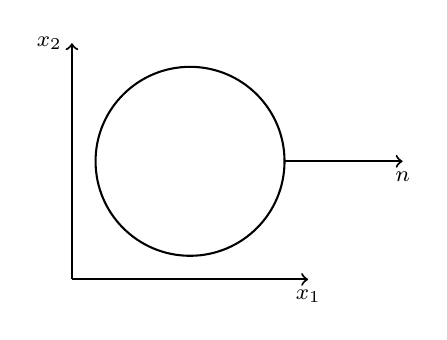
\begin{tikzpicture}[scale=3]
		
		\def \xone{0};
		\def \yone{0};		
		% draw coordinate system
		\coordinate (A) at (\xone,\yone);
		
		\draw[->] (A) -- ++(0,1);
		\draw[->] (A) -- ++(1,0);
		\draw[->] (A) ++(0.9,0.5) -- ++(0.5,0);

		% a circle is easier to draw than another object
        \draw (A) ++(0.5,0.5) circle (0.4cm);
        
        \fill[black,font=\footnotesize] (A) ++(1,0) node[below] {$x_{1}$}
										(A) ++(0,1) node[left] {$x_{2}$}
										(A) ++(1.4,0.5) node[below] {$n$};
                                        
\end{tikzpicture}

\caption{example $\Omega$,  $n$   outer normal on $\partial \Omega$}
\label{first picture}
\end{figure}

n outer normal on $\partial \Omega$
with boundary conditions
\[
\alpha u + \beta \frac{\partial u}{\partial n} = g \qquad \text{ on } \partial \Omega
.\] 

If \begin{itemize}
	\item $ \beta = 0$ and $\alpha=0$, we get a Dirichlet problem.
	\item  $\beta \neq 0$ and $ \alpha = 0$, we get a general Neumann problem.
	\item $\beta = 1$ and $\alpha = 0$, we have
		\begin{enumerate}
			\item Since $u = \text{const}$ solves \href{eq:eq_1}{(1)} 
				for $f=0 \text{ and } g = 0$, the solution to \href{eq:eq_1}{(1)} is unique up to a constant
			\item Integrating \href{eq:eq_1}{(1)} over $\Omega$ and Green's formula yield
				\[
				- \int_{\partial\Omega} \frac{\partial u}{\partial n} = - \int_{\Omega} \laplace u = \int_{\Omega} f
				.\] 
				This means, we get a compatibility condition
				\[
				\int_{\partial \Omega} g + \int_{\Omega}f = 0
				.\] 
		\end{enumerate}
\end{itemize} 

Another variant of \href{eq:eq_1}{(1)} is
\[
	Lu := \nabla(A\nabla u)
.\] 
where A is a positive definite matrix.

\begin{equation} \label{eq:eq_2}\tag{2}
LU = f \qquad \in \Omega \text{ + boundary condition}
\end{equation}

\section{Discretization with finite differences}%
\label{sec:Discretization with finite differences}

The basic idea is:

\begin{itemize}
	\item local approximation of partial derivatives
	\item derived by low order Taylor series
\end{itemize}

\begin{itemize}
	\item \underline{(1D-case):} 
		\[
			u'(x) \approx \frac{u(x+h)-u(x)}{h} = \delta^{+}u(x) \qquad \text{(forward difference)}
		.\] 
		For functions $u \in C^{4}$ in a neighbourhood of $x$, we get by Taylor's formula:
		\begin{equation} \label{eq:eq_3} \tag{$\ast$}
			u(x+h) = u(x) + h u'(x) + \frac{h^{2}}{2} u''(x) + \frac{h^{3}}{6}u'''(x) + \frac{h^{4}}{24}u''''(\xi_{+})	
		\end{equation}
		for some $\xi_{+} \in (x, x+h)$. Rearranging the equation gives
		\[
			u'(x) = \frac{u(x+h)-u(x)}{h}-\frac{h}{2}u''(x) + \O(h^{2})
		.\] 
		Now we plug this in in \href{eq:eq_4}{($\ast$)} and replace $h$ by $-h$ to get
		\begin{equation} \label{eq:eq_4} \tag{$\ast \ast$}
			u(x-h) = u(x) - hu'(x) + \frac{h^{2}}{2}u''(x)- \frac{h^{3}}{6} u'''(x) + \frac{h^{4}}{24}u''''(\xi _{-})
		\end{equation}
		For some appropriate $\xi _{-} \in (x-h, x)$.
		Adding up \href{eq:eq_3}{($\ast$)} and \href{eq:eq_4}{($\ast \ast)$} yields
		\[
			u''(x)= \frac{u(x+h) - 2u(x) + u(x-h)}{h^{2}} + \frac{h^{2}}{12}u''''(\xi )
		.\] for some $\xi  \in [\xi _{-}, \xi _{+}]$

		This is called the central difference approximation of the second order derivative.
		
		Let
		\[
			u'(x) \approx \frac{u(x)-u(x-h)}{h} = \delta^{-}u(x) \qquad \text{(backward difference)}
		.\] Then $u''(x) \approx \delta^{-}\delta^{+}u(x)$.

		For the elliptic operator $L:=\partial_{x} \Big(a(x)\partial_{x}\Big)$ we get a second order accurate formula by evaluating $a(x)$ inside the intervals $(x-h, x)$ and $(x, x+h)$
		\begin{align*}
			\partial_{x}(a(x) \partial_{x}u) &=
			\delta^{+}\Big(a(x- \frac{h}{2}) \delta^{-} u\Big) + \O(h^{2}) \\
											 &\approx \frac{a(x+\frac{h}{2})\Big(u(x+h)-u(x)\Big)-a(x-\frac{h}{2})\Big(u(x)-u(x-h)\Big)}{h^{2}}
		\end{align*}
		with $a(x \pm \frac{h}{2})$ either evaluated directly or by the average
		\[
			a(x \pm \frac{h}{2}) \approx \frac{1}{2}\Big(a(x \pm h) - a(x)\Big)
		.\] 
		
	\item \underline{(2D \& 3D cases):} 
		The laplacian is the sum of all second derivatives
		\[
			\laplace = \partial x_1^2 + \partial x_2^2 (+\partial x_3^2)
		.\] 
		With (possibly) different step width $h$ in each coordinate direction we get
		\begin{align*}
			\laplace u(x) &\approx \frac{u(x_1 + h_1, x_2) - 2u(x_1, x_2) + u(x_1 -h_1, x_2)}{h_1^2}\\
						  &+ \frac{u(x_1, x_2 + h_2) - 2u(x_1, x_2) + u(x_1, x_2 -h_2)}{h_2^2}
		\end{align*}
		but for $h_1 = h_2 = h$ we get
		\begin{align*}
			&\laplace u(x) \approx\\ 
			&\frac{1}{h^2}\left[u(x_1+ h, x_2) + u(x_1-h, x_2) + u(x_1, x_2 -h) + u(x_1, x_2 -h) -4u(x_1, x_2)\right].
		\end{align*}
		Denoting the forward/backward difference formulas
		in the direction i by $\delta_{i}^{+}$ and $\delta_{i}^{-}$ we can write
		\[
			\laplace u(x) \approx \sum_{i=1}^{2}{\delta_{i}^{+}\delta_{i}^{-}u(x)}=:\laplace_{h}^{(5)}u(x)
		.\] 
		The formula can be sketched as a stencil, the so called " 5-point stencil "
		\tikzset
{
	treenode/.style = {circle, draw=black!60, fill=white!40, very thick, minimum size=6mm}
}

\begin{figure}[H]
	\center

	\begin{tikzpicture}%[level/.style={sibling distance = 2cm/#1, level distance = 3cm}]
	
	\def \xone{0};
	\def \yone{0};
	
	\coordinate (root) at (\xone ,\yone);
	\draw (root) ++ (-1,0) -- ++(2,0);
	\draw (root) ++ (0,-1) -- ++(0,2);

	%draw nodes
	\node [treenode] at (root) {-4};
	\node [treenode] at (root) ++ (-1,0) {1};
	\node [treenode] at (root) ++ (1,0) {1};
	\node [treenode] at (root) ++ (0,1) {1};
	\node [treenode] at (root) ++ (0,-1) {1};

		
	\end{tikzpicture}
	
\caption{5-point stencil (second order accurate)}
\label{five_point}
\end{figure}

		where the values in the nodes correspond to the coefficients in the formula.
		Other possible stencils are:
		\begin{itemize}
			\item rotated 5-point-stencil, $2^{\text{nd}}$ order accurate
				\begin{figure}[H]
	\center

	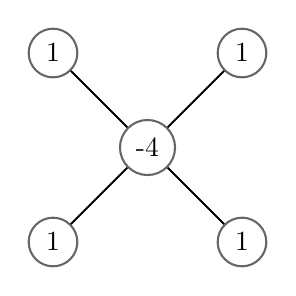
\begin{tikzpicture}

	\def \xone{0};
	\def \yone{0};
	\def \h{1.2}	

	\coordinate (M) at (\xone ,\yone);
	\coordinate (LU) at (\xone-\h ,\yone-\h);
	\coordinate (RU) at (\xone+\h ,\yone-\h);
	\coordinate (LO) at (\xone-\h ,\yone+\h);
	\coordinate (RO) at (\xone+\h ,\yone+\h);
	\draw (LU) -- (RO);
	\draw (RU) -- (LO);

	%draw nodes
	\node[circle,draw=black!60, fill=white!40] at (M) {-4};
	\node[circle,draw=black!60, fill=white!40] at (LO) {1};
	\node[circle,draw=black!60, fill=white!40] at (RO) {1};
	\node[circle,draw=black!60, fill=white!40] at (LU) {1};
	\node[circle,draw=black!60, fill=white!40] at (RU) {1};

		
	\end{tikzpicture}
\caption{rotated 5-point stencil}
\label{five_point_rot}
	
\end{figure}

			\item 9-point-stencil,  $2^{\text{nd}}$ order accurate and even $6^{\text{th}}$ order accurate for harmonic functions
				\begin{figure}[H]
	\center

	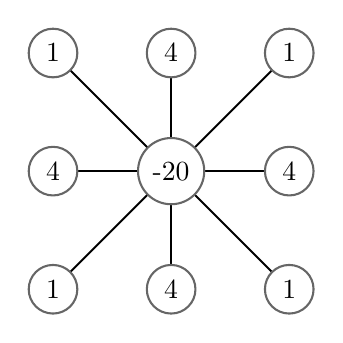
\begin{tikzpicture}
	
	\def \xone{0};
	\def \yone{0};
	\def \h{1.5}	

	\coordinate (M) at (\xone ,\yone);
	\coordinate (L) at (\xone-\h ,\yone);
	\coordinate (R) at (\xone+\h ,\yone);
	\coordinate (O) at (\xone ,\yone+\h);
	\coordinate (LU) at (\xone-\h ,\yone-\h);
	\coordinate (RU) at (\xone+\h ,\yone-\h);
	\coordinate (LO) at (\xone-\h ,\yone+\h);
	\coordinate (RO) at (\xone+\h ,\yone+\h);
	\coordinate (U) at (\xone ,\yone-\h);

	\draw (L) -- (R);
	\draw (U) -- (O);
	\draw (LU) -- (RO);
	\draw (RU) -- (LO);

	%draw nodes
	\node[circle,draw=black!60, fill=white!40] at (M) {-20};
	\node[circle,draw=black!60, fill=white!40] at (L) {4};
	\node[circle,draw=black!60, fill=white!40] at (R) {4};
	\node[circle,draw=black!60, fill=white!40] at (O) {4};
	\node[circle,draw=black!60, fill=white!40] at (U) {4};

	%draw diagonal nodes
	\node[circle,draw=black!60, fill=white!40] at (LO) {1};
	\node[circle,draw=black!60, fill=white!40] at (RO) {1};
	\node[circle,draw=black!60, fill=white!40] at (LU) {1};
	\node[circle,draw=black!60, fill=white!40] at (RU) {1};

	
	\end{tikzpicture}
	\caption{9-point stencil}
\label{nine_point}
	
\end{figure}

		\end{itemize}
\end{itemize}

\section{Finite difference on a grid}%
\label{sec:Finite difference on a grid}
Let $\Omega =(0, X_{E}) \times (0,Y_{E})$ and subdivide each interval into $N_{x}+1 / N_{y} + 1$ subintervals.

\[
\left.
	\begin{array}{c}
	N_{x} = 1 \\
	N_{y} = 2
\end{array}
\right\} \qquad
h_{x} = \frac{x_{E}}{N_{x}+1}, \quad h_{y}= \frac{y_{E}}{N_{y}+1}
.\] 

\begin{figure}[H]
	\center
\begin{tikzpicture}[scale=3]
		
		\def \xone{0};
		\def \yone{0};		
		% draw coordinate system
		\coordinate (A) at (\xone,\yone);
		
		\draw[\to] (A) -- ++(0,1);
		\draw[\to] (A) -- ++(1,0);
		\draw (A) ++(0.5,0) -- ++ (0,1);
		\draw (A) ++(1,0) -- ++ (0,1) -- ++(-1,0);
		\draw (A) ++(0,0.333) -- ++ (1,0);
		\draw (A) ++(0,0.666) -- ++ (1,0);
		\draw[red!60] (A) -- (A) ++ (0,0.333);
		\draw[blue!60] (A) -- (A) ++ (0.5,0);

        \fill[black,font=\footnotesize] (A)  ++(1,0) node[under] {$x_{E}$}
										(A)  ++(0,1) node[left] {$y_{E}$}
										(A)  ++(0.25,0) node[under] {$h_{x}$}
										(A)  ++(0,0.1666) node[left] {$h_{y}$};
                                        
\end{tikzpicture}

\caption{Visualization of Grid}
\label{example_grid}
\end{figure}

Each node (vertex) in this grid is assigned an index tuple
\[
	(x,y) = (ih_{x}, jh_{y}) \stackeq{\wedge} (i,j)
.\] 
for $i \in \{0,1, \ldots , N_{x}+1\}, j \in  \{0,1, \ldots , N_{y}+1\}$

We denote the value at the node $(i,j)$ by
\[
	u(x,y)=u(ih_{x},jh_{y})=:u_{i,j}
.\] 
This results in the discrete Laplace operator $(h=h_{x}=h_{y})$
\[
	\laplace_{h}^{(5)}u_{i,j}=\frac{1}{2}(u_{i+1,j}+u_{i-1,j} +u_{i,j+1}+ u_{i,j-1} - 4u_{i,j})
.\]

\newpage
\section{Node ordering}%
\label{sec:Node ordering}
To form a linear system, the nodes $(i,j)$ have to be numbered consecutively, i.e. we have to use a map
\[
	l\colon \N^{d} \rightarrow \N
.\] 

Examples:

\begin{enumerate}[label=\alph{enumi})]
	\item  Lexicographical ordering
		\[
			l(i,j) = j \cdot (N_{x} + 2) + i 
			\quad\text{ or }\quad
			l(i,j) = i \cdot (N_{y} + 2) + j
		.\] 

		\begin{figure}[ht!]
			\begin{center}
				

\tikzset{every picture/.style={line width=0.75pt}} %set default line width to 0.75pt        

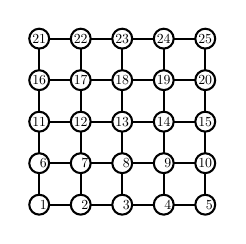
\begin{tikzpicture}[x=0.75pt,y=0.75pt,yscale=-1,xscale=1]
%uncomment if require: \path (0,214); %set diagram left start at 0, and has height of 214

%Shape: Grid [id:dp20427001490833852] 
\draw  [draw opacity=0][fill={rgb, 255:red, 255; green, 255; blue, 255 }  ,fill opacity=1 ] (289.5,62) -- (369.67,62) -- (369.67,142.5) -- (289.5,142.5) -- cycle ; \draw   (289.5,62) -- (289.5,142.5)(309.5,62) -- (309.5,142.5)(329.5,62) -- (329.5,142.5)(349.5,62) -- (349.5,142.5)(369.5,62) -- (369.5,142.5) ; \draw   (289.5,62) -- (369.67,62)(289.5,82) -- (369.67,82)(289.5,102) -- (369.67,102)(289.5,122) -- (369.67,122)(289.5,142) -- (369.67,142) ; \draw    ;
%Shape: Circle [id:dp7961893048519293] 
\draw  [fill={rgb, 255:red, 255; green, 255; blue, 255 }  ,fill opacity=1 ] (284.71,142) .. controls (284.71,139.35) and (286.85,137.21) .. (289.5,137.21) .. controls (292.15,137.21) and (294.29,139.35) .. (294.29,142) .. controls (294.29,144.65) and (292.15,146.79) .. (289.5,146.79) .. controls (286.85,146.79) and (284.71,144.65) .. (284.71,142) -- cycle ;
%Shape: Circle [id:dp11966537247793707] 
\draw  [fill={rgb, 255:red, 255; green, 255; blue, 255 }  ,fill opacity=1 ] (304.71,142) .. controls (304.71,139.35) and (306.85,137.21) .. (309.5,137.21) .. controls (312.15,137.21) and (314.29,139.35) .. (314.29,142) .. controls (314.29,144.65) and (312.15,146.79) .. (309.5,146.79) .. controls (306.85,146.79) and (304.71,144.65) .. (304.71,142) -- cycle ;
%Shape: Circle [id:dp10804608038481334] 
\draw  [fill={rgb, 255:red, 255; green, 255; blue, 255 }  ,fill opacity=1 ] (324.71,142) .. controls (324.71,139.35) and (326.85,137.21) .. (329.5,137.21) .. controls (332.15,137.21) and (334.29,139.35) .. (334.29,142) .. controls (334.29,144.65) and (332.15,146.79) .. (329.5,146.79) .. controls (326.85,146.79) and (324.71,144.65) .. (324.71,142) -- cycle ;
%Shape: Circle [id:dp09169839430121018] 
\draw  [fill={rgb, 255:red, 255; green, 255; blue, 255 }  ,fill opacity=1 ] (344.71,142) .. controls (344.71,139.35) and (346.85,137.21) .. (349.5,137.21) .. controls (352.15,137.21) and (354.29,139.35) .. (354.29,142) .. controls (354.29,144.65) and (352.15,146.79) .. (349.5,146.79) .. controls (346.85,146.79) and (344.71,144.65) .. (344.71,142) -- cycle ;
%Shape: Circle [id:dp583721092220175] 
\draw  [fill={rgb, 255:red, 255; green, 255; blue, 255 }  ,fill opacity=1 ] (364.71,142) .. controls (364.71,139.35) and (366.85,137.21) .. (369.5,137.21) .. controls (372.15,137.21) and (374.29,139.35) .. (374.29,142) .. controls (374.29,144.65) and (372.15,146.79) .. (369.5,146.79) .. controls (366.85,146.79) and (364.71,144.65) .. (364.71,142) -- cycle ;
%Shape: Circle [id:dp7957737292663944] 
\draw  [fill={rgb, 255:red, 255; green, 255; blue, 255 }  ,fill opacity=1 ] (364.71,102) .. controls (364.71,99.35) and (366.85,97.21) .. (369.5,97.21) .. controls (372.15,97.21) and (374.29,99.35) .. (374.29,102) .. controls (374.29,104.65) and (372.15,106.79) .. (369.5,106.79) .. controls (366.85,106.79) and (364.71,104.65) .. (364.71,102) -- cycle ;
%Shape: Circle [id:dp4337691692976733] 
\draw  [fill={rgb, 255:red, 255; green, 255; blue, 255 }  ,fill opacity=1 ] (364.71,122) .. controls (364.71,119.35) and (366.85,117.21) .. (369.5,117.21) .. controls (372.15,117.21) and (374.29,119.35) .. (374.29,122) .. controls (374.29,124.65) and (372.15,126.79) .. (369.5,126.79) .. controls (366.85,126.79) and (364.71,124.65) .. (364.71,122) -- cycle ;
%Shape: Circle [id:dp6938306155681562] 
\draw  [fill={rgb, 255:red, 255; green, 255; blue, 255 }  ,fill opacity=1 ] (344.71,122) .. controls (344.71,119.35) and (346.85,117.21) .. (349.5,117.21) .. controls (352.15,117.21) and (354.29,119.35) .. (354.29,122) .. controls (354.29,124.65) and (352.15,126.79) .. (349.5,126.79) .. controls (346.85,126.79) and (344.71,124.65) .. (344.71,122) -- cycle ;
%Shape: Circle [id:dp7383635507732627] 
\draw  [fill={rgb, 255:red, 255; green, 255; blue, 255 }  ,fill opacity=1 ] (324.71,122) .. controls (324.71,119.35) and (326.85,117.21) .. (329.5,117.21) .. controls (332.15,117.21) and (334.29,119.35) .. (334.29,122) .. controls (334.29,124.65) and (332.15,126.79) .. (329.5,126.79) .. controls (326.85,126.79) and (324.71,124.65) .. (324.71,122) -- cycle ;
%Shape: Circle [id:dp0688209668837807] 
\draw  [fill={rgb, 255:red, 255; green, 255; blue, 255 }  ,fill opacity=1 ] (304.71,122) .. controls (304.71,119.35) and (306.85,117.21) .. (309.5,117.21) .. controls (312.15,117.21) and (314.29,119.35) .. (314.29,122) .. controls (314.29,124.65) and (312.15,126.79) .. (309.5,126.79) .. controls (306.85,126.79) and (304.71,124.65) .. (304.71,122) -- cycle ;
%Shape: Circle [id:dp7530655534187332] 
\draw  [fill={rgb, 255:red, 255; green, 255; blue, 255 }  ,fill opacity=1 ] (284.71,122) .. controls (284.71,119.35) and (286.85,117.21) .. (289.5,117.21) .. controls (292.15,117.21) and (294.29,119.35) .. (294.29,122) .. controls (294.29,124.65) and (292.15,126.79) .. (289.5,126.79) .. controls (286.85,126.79) and (284.71,124.65) .. (284.71,122) -- cycle ;
%Shape: Circle [id:dp3625747513152686] 
\draw  [fill={rgb, 255:red, 255; green, 255; blue, 255 }  ,fill opacity=1 ] (284.71,102) .. controls (284.71,99.35) and (286.85,97.21) .. (289.5,97.21) .. controls (292.15,97.21) and (294.29,99.35) .. (294.29,102) .. controls (294.29,104.65) and (292.15,106.79) .. (289.5,106.79) .. controls (286.85,106.79) and (284.71,104.65) .. (284.71,102) -- cycle ;
%Shape: Circle [id:dp6795946046973622] 
\draw  [fill={rgb, 255:red, 255; green, 255; blue, 255 }  ,fill opacity=1 ] (304.71,102) .. controls (304.71,99.35) and (306.85,97.21) .. (309.5,97.21) .. controls (312.15,97.21) and (314.29,99.35) .. (314.29,102) .. controls (314.29,104.65) and (312.15,106.79) .. (309.5,106.79) .. controls (306.85,106.79) and (304.71,104.65) .. (304.71,102) -- cycle ;
%Shape: Circle [id:dp41690154167403715] 
\draw  [fill={rgb, 255:red, 255; green, 255; blue, 255 }  ,fill opacity=1 ] (324.71,102) .. controls (324.71,99.35) and (326.85,97.21) .. (329.5,97.21) .. controls (332.15,97.21) and (334.29,99.35) .. (334.29,102) .. controls (334.29,104.65) and (332.15,106.79) .. (329.5,106.79) .. controls (326.85,106.79) and (324.71,104.65) .. (324.71,102) -- cycle ;
%Shape: Circle [id:dp12388036817192649] 
\draw  [fill={rgb, 255:red, 255; green, 255; blue, 255 }  ,fill opacity=1 ] (344.71,102) .. controls (344.71,99.35) and (346.85,97.21) .. (349.5,97.21) .. controls (352.15,97.21) and (354.29,99.35) .. (354.29,102) .. controls (354.29,104.65) and (352.15,106.79) .. (349.5,106.79) .. controls (346.85,106.79) and (344.71,104.65) .. (344.71,102) -- cycle ;
%Shape: Circle [id:dp020335686116125018] 
\draw  [fill={rgb, 255:red, 255; green, 255; blue, 255 }  ,fill opacity=1 ] (284.71,82) .. controls (284.71,79.35) and (286.85,77.21) .. (289.5,77.21) .. controls (292.15,77.21) and (294.29,79.35) .. (294.29,82) .. controls (294.29,84.65) and (292.15,86.79) .. (289.5,86.79) .. controls (286.85,86.79) and (284.71,84.65) .. (284.71,82) -- cycle ;
%Shape: Circle [id:dp8773782628717408] 
\draw  [fill={rgb, 255:red, 255; green, 255; blue, 255 }  ,fill opacity=1 ] (304.71,82) .. controls (304.71,79.35) and (306.85,77.21) .. (309.5,77.21) .. controls (312.15,77.21) and (314.29,79.35) .. (314.29,82) .. controls (314.29,84.65) and (312.15,86.79) .. (309.5,86.79) .. controls (306.85,86.79) and (304.71,84.65) .. (304.71,82) -- cycle ;
%Shape: Circle [id:dp6914481318920651] 
\draw  [fill={rgb, 255:red, 255; green, 255; blue, 255 }  ,fill opacity=1 ] (324.71,82) .. controls (324.71,79.35) and (326.85,77.21) .. (329.5,77.21) .. controls (332.15,77.21) and (334.29,79.35) .. (334.29,82) .. controls (334.29,84.65) and (332.15,86.79) .. (329.5,86.79) .. controls (326.85,86.79) and (324.71,84.65) .. (324.71,82) -- cycle ;
%Shape: Circle [id:dp48750295365917884] 
\draw  [fill={rgb, 255:red, 255; green, 255; blue, 255 }  ,fill opacity=1 ] (344.71,82) .. controls (344.71,79.35) and (346.85,77.21) .. (349.5,77.21) .. controls (352.15,77.21) and (354.29,79.35) .. (354.29,82) .. controls (354.29,84.65) and (352.15,86.79) .. (349.5,86.79) .. controls (346.85,86.79) and (344.71,84.65) .. (344.71,82) -- cycle ;
%Shape: Circle [id:dp39103551666768044] 
\draw  [fill={rgb, 255:red, 255; green, 255; blue, 255 }  ,fill opacity=1 ] (364.71,82) .. controls (364.71,79.35) and (366.85,77.21) .. (369.5,77.21) .. controls (372.15,77.21) and (374.29,79.35) .. (374.29,82) .. controls (374.29,84.65) and (372.15,86.79) .. (369.5,86.79) .. controls (366.85,86.79) and (364.71,84.65) .. (364.71,82) -- cycle ;
%Shape: Circle [id:dp7705867635318655] 
\draw  [fill={rgb, 255:red, 255; green, 255; blue, 255 }  ,fill opacity=1 ] (284.71,62) .. controls (284.71,59.35) and (286.85,57.21) .. (289.5,57.21) .. controls (292.15,57.21) and (294.29,59.35) .. (294.29,62) .. controls (294.29,64.65) and (292.15,66.79) .. (289.5,66.79) .. controls (286.85,66.79) and (284.71,64.65) .. (284.71,62) -- cycle ;
%Shape: Circle [id:dp989295643349072] 
\draw  [fill={rgb, 255:red, 255; green, 255; blue, 255 }  ,fill opacity=1 ] (304.71,62) .. controls (304.71,59.35) and (306.85,57.21) .. (309.5,57.21) .. controls (312.15,57.21) and (314.29,59.35) .. (314.29,62) .. controls (314.29,64.65) and (312.15,66.79) .. (309.5,66.79) .. controls (306.85,66.79) and (304.71,64.65) .. (304.71,62) -- cycle ;
%Shape: Circle [id:dp39113070395348526] 
\draw  [fill={rgb, 255:red, 255; green, 255; blue, 255 }  ,fill opacity=1 ] (324.71,62) .. controls (324.71,59.35) and (326.85,57.21) .. (329.5,57.21) .. controls (332.15,57.21) and (334.29,59.35) .. (334.29,62) .. controls (334.29,64.65) and (332.15,66.79) .. (329.5,66.79) .. controls (326.85,66.79) and (324.71,64.65) .. (324.71,62) -- cycle ;
%Shape: Circle [id:dp001355361767774177] 
\draw  [fill={rgb, 255:red, 255; green, 255; blue, 255 }  ,fill opacity=1 ] (344.71,62) .. controls (344.71,59.35) and (346.85,57.21) .. (349.5,57.21) .. controls (352.15,57.21) and (354.29,59.35) .. (354.29,62) .. controls (354.29,64.65) and (352.15,66.79) .. (349.5,66.79) .. controls (346.85,66.79) and (344.71,64.65) .. (344.71,62) -- cycle ;
%Shape: Circle [id:dp3504756976635919] 
\draw  [fill={rgb, 255:red, 255; green, 255; blue, 255 }  ,fill opacity=1 ] (364.71,62) .. controls (364.71,59.35) and (366.85,57.21) .. (369.5,57.21) .. controls (372.15,57.21) and (374.29,59.35) .. (374.29,62) .. controls (374.29,64.65) and (372.15,66.79) .. (369.5,66.79) .. controls (366.85,66.79) and (364.71,64.65) .. (364.71,62) -- cycle ;

% Text Node
\draw (291.5,142) node [scale=0.5] [align=left] {1};
% Text Node
\draw (311.5,142) node [scale=0.5] [align=left] {2};
% Text Node
\draw (331.5,142) node [scale=0.5] [align=left] {3};
% Text Node
\draw (351.5,142) node [scale=0.5] [align=left] {4};
% Text Node
\draw (371.5,142) node [scale=0.5] [align=left] {5};
% Text Node
\draw (291.5,122) node [scale=0.5] [align=left] {6};
% Text Node
\draw (311.5,122) node [scale=0.5] [align=left] {7};
% Text Node
\draw (331.5,122) node [scale=0.5] [align=left] {8};
% Text Node
\draw (351.5,122) node [scale=0.5] [align=left] {9};
% Text Node
\draw (369.5,122) node [scale=0.5] [align=left] {10};
% Text Node
\draw (289.5,102) node [scale=0.5] [align=left] {11};
% Text Node
\draw (309.5,102) node [scale=0.5] [align=left] {12};
% Text Node
\draw (329.5,102) node [scale=0.5] [align=left] {13};
% Text Node
\draw (349.5,102) node [scale=0.5] [align=left] {14};
% Text Node
\draw (369.5,102) node [scale=0.5] [align=left] {15};
% Text Node
\draw (289.5,82) node [scale=0.5] [align=left] {16};
% Text Node
\draw (309.5,82) node [scale=0.5] [align=left] {17};
% Text Node
\draw (329.5,82) node [scale=0.5] [align=left] {18};
% Text Node
\draw (349.5,82) node [scale=0.5] [align=left] {19};
% Text Node
\draw (369.5,82) node [scale=0.5] [align=left] {20};
% Text Node
\draw (289.5,62) node [scale=0.5] [align=left] {21};
% Text Node
\draw (309.5,62) node [scale=0.5] [align=left] {22};
% Text Node
\draw (329.5,62) node [scale=0.5] [align=left] {23};
% Text Node
\draw (349.5,62) node [scale=0.5] [align=left] {24};
% Text Node
\draw (369.5,62) node [scale=0.5] [align=left] {25};


\end{tikzpicture}

			\end{center}
			\caption{Lexicographical ordering}
			\label{fig:lexiorder}
		\end{figure}
		
	\item Red-Black ordering (checkerboard ordering)

		\begin{enumerate}[label=\arabic{enumii})]
			\item neighbouring nodes get different color
			\item number each node lexicographically
		\end{enumerate}

		\begin{figure}[ht!]
			\begin{center}
				

\tikzset{every picture/.style={line width=0.75pt}} %set default line width to 0.75pt        

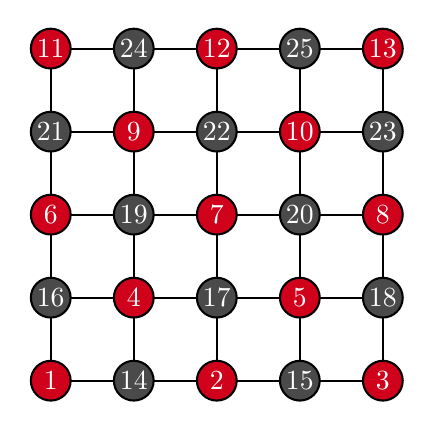
\begin{tikzpicture}[x=0.75pt,y=0.75pt,yscale=-2,xscale=2]
%uncomment if require: \path (0,222); %set diagram left start at 0, and has height of 222

%Shape: Grid [id:dp7509010194001084] 
\draw  [draw opacity=0][fill={rgb, 255:red, 255; green, 255; blue, 255 }  ,fill opacity=1 ] (289.5,76) -- (369.67,76) -- (369.67,156.5) -- (289.5,156.5) -- cycle ; \draw   (289.5,76) -- (289.5,156.5)(309.5,76) -- (309.5,156.5)(329.5,76) -- (329.5,156.5)(349.5,76) -- (349.5,156.5)(369.5,76) -- (369.5,156.5) ; \draw   (289.5,76) -- (369.67,76)(289.5,96) -- (369.67,96)(289.5,116) -- (369.67,116)(289.5,136) -- (369.67,136)(289.5,156) -- (369.67,156) ; \draw    ;
%Shape: Circle [id:dp6108755291859196] 
\draw  [fill={rgb, 255:red, 208; green, 2; blue, 27 }  ,fill opacity=1 ] (284.71,156) .. controls (284.71,153.35) and (286.85,151.21) .. (289.5,151.21) .. controls (292.15,151.21) and (294.29,153.35) .. (294.29,156) .. controls (294.29,158.65) and (292.15,160.79) .. (289.5,160.79) .. controls (286.85,160.79) and (284.71,158.65) .. (284.71,156) -- cycle ;
%Shape: Circle [id:dp4441687082516983] 
\draw  [fill={rgb, 255:red, 74; green, 74; blue, 74 }  ,fill opacity=1 ] (304.71,156) .. controls (304.71,153.35) and (306.85,151.21) .. (309.5,151.21) .. controls (312.15,151.21) and (314.29,153.35) .. (314.29,156) .. controls (314.29,158.65) and (312.15,160.79) .. (309.5,160.79) .. controls (306.85,160.79) and (304.71,158.65) .. (304.71,156) -- cycle ;
%Shape: Circle [id:dp6167896316379069] 
\draw  [fill={rgb, 255:red, 208; green, 2; blue, 27 }  ,fill opacity=1 ] (324.71,156) .. controls (324.71,153.35) and (326.85,151.21) .. (329.5,151.21) .. controls (332.15,151.21) and (334.29,153.35) .. (334.29,156) .. controls (334.29,158.65) and (332.15,160.79) .. (329.5,160.79) .. controls (326.85,160.79) and (324.71,158.65) .. (324.71,156) -- cycle ;
%Shape: Circle [id:dp6715236044117903] 
\draw  [fill={rgb, 255:red, 74; green, 74; blue, 74 }  ,fill opacity=1 ] (344.71,156) .. controls (344.71,153.35) and (346.85,151.21) .. (349.5,151.21) .. controls (352.15,151.21) and (354.29,153.35) .. (354.29,156) .. controls (354.29,158.65) and (352.15,160.79) .. (349.5,160.79) .. controls (346.85,160.79) and (344.71,158.65) .. (344.71,156) -- cycle ;
%Shape: Circle [id:dp06410493254248473] 
\draw  [fill={rgb, 255:red, 208; green, 2; blue, 27 }  ,fill opacity=1 ] (364.71,156) .. controls (364.71,153.35) and (366.85,151.21) .. (369.5,151.21) .. controls (372.15,151.21) and (374.29,153.35) .. (374.29,156) .. controls (374.29,158.65) and (372.15,160.79) .. (369.5,160.79) .. controls (366.85,160.79) and (364.71,158.65) .. (364.71,156) -- cycle ;
%Shape: Circle [id:dp6649764858783351] 
\draw  [fill={rgb, 255:red, 208; green, 2; blue, 27 }  ,fill opacity=1 ] (364.71,116) .. controls (364.71,113.35) and (366.85,111.21) .. (369.5,111.21) .. controls (372.15,111.21) and (374.29,113.35) .. (374.29,116) .. controls (374.29,118.65) and (372.15,120.79) .. (369.5,120.79) .. controls (366.85,120.79) and (364.71,118.65) .. (364.71,116) -- cycle ;
%Shape: Circle [id:dp9554900297815432] 
\draw  [fill={rgb, 255:red, 74; green, 74; blue, 74 }  ,fill opacity=1 ] (364.71,136) .. controls (364.71,133.35) and (366.85,131.21) .. (369.5,131.21) .. controls (372.15,131.21) and (374.29,133.35) .. (374.29,136) .. controls (374.29,138.65) and (372.15,140.79) .. (369.5,140.79) .. controls (366.85,140.79) and (364.71,138.65) .. (364.71,136) -- cycle ;
%Shape: Circle [id:dp37112581806137124] 
\draw  [fill={rgb, 255:red, 208; green, 2; blue, 27 }  ,fill opacity=1 ] (344.71,136) .. controls (344.71,133.35) and (346.85,131.21) .. (349.5,131.21) .. controls (352.15,131.21) and (354.29,133.35) .. (354.29,136) .. controls (354.29,138.65) and (352.15,140.79) .. (349.5,140.79) .. controls (346.85,140.79) and (344.71,138.65) .. (344.71,136) -- cycle ;
%Shape: Circle [id:dp06306680838602707] 
\draw  [fill={rgb, 255:red, 74; green, 74; blue, 74 }  ,fill opacity=1 ] (324.71,136) .. controls (324.71,133.35) and (326.85,131.21) .. (329.5,131.21) .. controls (332.15,131.21) and (334.29,133.35) .. (334.29,136) .. controls (334.29,138.65) and (332.15,140.79) .. (329.5,140.79) .. controls (326.85,140.79) and (324.71,138.65) .. (324.71,136) -- cycle ;
%Shape: Circle [id:dp9358022961380756] 
\draw  [fill={rgb, 255:red, 208; green, 2; blue, 27 }  ,fill opacity=1 ] (304.71,136) .. controls (304.71,133.35) and (306.85,131.21) .. (309.5,131.21) .. controls (312.15,131.21) and (314.29,133.35) .. (314.29,136) .. controls (314.29,138.65) and (312.15,140.79) .. (309.5,140.79) .. controls (306.85,140.79) and (304.71,138.65) .. (304.71,136) -- cycle ;
%Shape: Circle [id:dp9068520178890649] 
\draw  [fill={rgb, 255:red, 74; green, 74; blue, 74 }  ,fill opacity=1 ] (284.71,136) .. controls (284.71,133.35) and (286.85,131.21) .. (289.5,131.21) .. controls (292.15,131.21) and (294.29,133.35) .. (294.29,136) .. controls (294.29,138.65) and (292.15,140.79) .. (289.5,140.79) .. controls (286.85,140.79) and (284.71,138.65) .. (284.71,136) -- cycle ;
%Shape: Circle [id:dp8562155796812134] 
\draw  [fill={rgb, 255:red, 208; green, 2; blue, 27 }  ,fill opacity=1 ] (284.71,116) .. controls (284.71,113.35) and (286.85,111.21) .. (289.5,111.21) .. controls (292.15,111.21) and (294.29,113.35) .. (294.29,116) .. controls (294.29,118.65) and (292.15,120.79) .. (289.5,120.79) .. controls (286.85,120.79) and (284.71,118.65) .. (284.71,116) -- cycle ;
%Shape: Circle [id:dp2479839382803859] 
\draw  [fill={rgb, 255:red, 74; green, 74; blue, 74 }  ,fill opacity=1 ] (304.71,116) .. controls (304.71,113.35) and (306.85,111.21) .. (309.5,111.21) .. controls (312.15,111.21) and (314.29,113.35) .. (314.29,116) .. controls (314.29,118.65) and (312.15,120.79) .. (309.5,120.79) .. controls (306.85,120.79) and (304.71,118.65) .. (304.71,116) -- cycle ;
%Shape: Circle [id:dp8339992993489453] 
\draw  [fill={rgb, 255:red, 208; green, 2; blue, 27 }  ,fill opacity=1 ] (324.71,116) .. controls (324.71,113.35) and (326.85,111.21) .. (329.5,111.21) .. controls (332.15,111.21) and (334.29,113.35) .. (334.29,116) .. controls (334.29,118.65) and (332.15,120.79) .. (329.5,120.79) .. controls (326.85,120.79) and (324.71,118.65) .. (324.71,116) -- cycle ;
%Shape: Circle [id:dp29657132974437017] 
\draw  [fill={rgb, 255:red, 74; green, 74; blue, 74 }  ,fill opacity=1 ] (344.71,116) .. controls (344.71,113.35) and (346.85,111.21) .. (349.5,111.21) .. controls (352.15,111.21) and (354.29,113.35) .. (354.29,116) .. controls (354.29,118.65) and (352.15,120.79) .. (349.5,120.79) .. controls (346.85,120.79) and (344.71,118.65) .. (344.71,116) -- cycle ;
%Shape: Circle [id:dp4006844726389853] 
\draw  [fill={rgb, 255:red, 74; green, 74; blue, 74 }  ,fill opacity=1 ] (284.71,96) .. controls (284.71,93.35) and (286.85,91.21) .. (289.5,91.21) .. controls (292.15,91.21) and (294.29,93.35) .. (294.29,96) .. controls (294.29,98.65) and (292.15,100.79) .. (289.5,100.79) .. controls (286.85,100.79) and (284.71,98.65) .. (284.71,96) -- cycle ;
%Shape: Circle [id:dp2518725902881924] 
\draw  [fill={rgb, 255:red, 208; green, 2; blue, 27 }  ,fill opacity=1 ] (304.71,96) .. controls (304.71,93.35) and (306.85,91.21) .. (309.5,91.21) .. controls (312.15,91.21) and (314.29,93.35) .. (314.29,96) .. controls (314.29,98.65) and (312.15,100.79) .. (309.5,100.79) .. controls (306.85,100.79) and (304.71,98.65) .. (304.71,96) -- cycle ;
%Shape: Circle [id:dp9478829895408571] 
\draw  [fill={rgb, 255:red, 74; green, 74; blue, 74 }  ,fill opacity=1 ] (324.71,96) .. controls (324.71,93.35) and (326.85,91.21) .. (329.5,91.21) .. controls (332.15,91.21) and (334.29,93.35) .. (334.29,96) .. controls (334.29,98.65) and (332.15,100.79) .. (329.5,100.79) .. controls (326.85,100.79) and (324.71,98.65) .. (324.71,96) -- cycle ;
%Shape: Circle [id:dp5111042484735311] 
\draw  [fill={rgb, 255:red, 208; green, 2; blue, 27 }  ,fill opacity=1 ] (344.71,96) .. controls (344.71,93.35) and (346.85,91.21) .. (349.5,91.21) .. controls (352.15,91.21) and (354.29,93.35) .. (354.29,96) .. controls (354.29,98.65) and (352.15,100.79) .. (349.5,100.79) .. controls (346.85,100.79) and (344.71,98.65) .. (344.71,96) -- cycle ;
%Shape: Circle [id:dp08226041749176072] 
\draw  [fill={rgb, 255:red, 74; green, 74; blue, 74 }  ,fill opacity=1 ] (364.71,96) .. controls (364.71,93.35) and (366.85,91.21) .. (369.5,91.21) .. controls (372.15,91.21) and (374.29,93.35) .. (374.29,96) .. controls (374.29,98.65) and (372.15,100.79) .. (369.5,100.79) .. controls (366.85,100.79) and (364.71,98.65) .. (364.71,96) -- cycle ;
%Shape: Circle [id:dp6793036732090996] 
\draw  [fill={rgb, 255:red, 208; green, 2; blue, 27 }  ,fill opacity=1 ] (284.71,76) .. controls (284.71,73.35) and (286.85,71.21) .. (289.5,71.21) .. controls (292.15,71.21) and (294.29,73.35) .. (294.29,76) .. controls (294.29,78.65) and (292.15,80.79) .. (289.5,80.79) .. controls (286.85,80.79) and (284.71,78.65) .. (284.71,76) -- cycle ;
%Shape: Circle [id:dp4959600894339744] 
\draw  [fill={rgb, 255:red, 74; green, 74; blue, 74 }  ,fill opacity=1 ] (304.71,76) .. controls (304.71,73.35) and (306.85,71.21) .. (309.5,71.21) .. controls (312.15,71.21) and (314.29,73.35) .. (314.29,76) .. controls (314.29,78.65) and (312.15,80.79) .. (309.5,80.79) .. controls (306.85,80.79) and (304.71,78.65) .. (304.71,76) -- cycle ;
%Shape: Circle [id:dp9621563131775881] 
\draw  [fill={rgb, 255:red, 208; green, 2; blue, 27 }  ,fill opacity=1 ] (324.71,76) .. controls (324.71,73.35) and (326.85,71.21) .. (329.5,71.21) .. controls (332.15,71.21) and (334.29,73.35) .. (334.29,76) .. controls (334.29,78.65) and (332.15,80.79) .. (329.5,80.79) .. controls (326.85,80.79) and (324.71,78.65) .. (324.71,76) -- cycle ;
%Shape: Circle [id:dp06302816821338242] 
\draw  [fill={rgb, 255:red, 74; green, 74; blue, 74 }  ,fill opacity=1 ] (344.71,76) .. controls (344.71,73.35) and (346.85,71.21) .. (349.5,71.21) .. controls (352.15,71.21) and (354.29,73.35) .. (354.29,76) .. controls (354.29,78.65) and (352.15,80.79) .. (349.5,80.79) .. controls (346.85,80.79) and (344.71,78.65) .. (344.71,76) -- cycle ;
%Shape: Circle [id:dp40969700298757994] 
\draw  [fill={rgb, 255:red, 208; green, 2; blue, 27 }  ,fill opacity=1 ] (364.71,76) .. controls (364.71,73.35) and (366.85,71.21) .. (369.5,71.21) .. controls (372.15,71.21) and (374.29,73.35) .. (374.29,76) .. controls (374.29,78.65) and (372.15,80.79) .. (369.5,80.79) .. controls (366.85,80.79) and (364.71,78.65) .. (364.71,76) -- cycle ;

% Text Node
\draw (289.5,156) node [scale=1,color={rgb, 255:red, 255; green, 255; blue, 255 }  ,opacity=1 ] [align=left] {1};
% Text Node
\draw (329.5,156) node [scale=1,color={rgb, 255:red, 255; green, 255; blue, 255 }  ,opacity=1 ] [align=left] {2};
% Text Node
\draw (369.5,156) node [scale=1,color={rgb, 255:red, 255; green, 255; blue, 255 }  ,opacity=1 ] [align=left] {3};
% Text Node
\draw (309.5,136) node [scale=1,color={rgb, 255:red, 255; green, 255; blue, 255 }  ,opacity=1 ] [align=left] {4};
% Text Node
\draw (349.5,136) node [scale=1,color={rgb, 255:red, 255; green, 255; blue, 255 }  ,opacity=1 ] [align=left] {5};
% Text Node
\draw (289.5,116) node [scale=1,color={rgb, 255:red, 255; green, 255; blue, 255 }  ,opacity=1 ] [align=left] {6};
% Text Node
\draw (329.5,116) node [scale=1,color={rgb, 255:red, 255; green, 255; blue, 255 }  ,opacity=1 ] [align=left] {7};
% Text Node
\draw (369.5,116) node [scale=1,color={rgb, 255:red, 255; green, 255; blue, 255 }  ,opacity=1 ] [align=left] {8};
% Text Node
\draw (309.5,96) node [scale=1,color={rgb, 255:red, 255; green, 255; blue, 255 }  ,opacity=1 ] [align=left] {9};
% Text Node
\draw (349.5,96) node [scale=1,color={rgb, 255:red, 255; green, 255; blue, 255 }  ,opacity=1 ] [align=left] {10};
% Text Node
\draw (289.5,76) node [scale=1,color={rgb, 255:red, 255; green, 255; blue, 255 }  ,opacity=1 ] [align=left] {11};
% Text Node
\draw (329.5,76) node [scale=1,color={rgb, 255:red, 255; green, 255; blue, 255 }  ,opacity=1 ] [align=left] {12};
% Text Node
\draw (369.5,76) node [scale=1,color={rgb, 255:red, 255; green, 255; blue, 255 }  ,opacity=1 ] [align=left] {13};
% Text Node
\draw (309.5,156) node [scale=1,color={rgb, 255:red, 255; green, 255; blue, 255 }  ,opacity=1 ] [align=left] {14};
% Text Node
\draw (349.5,156) node [scale=1,color={rgb, 255:red, 255; green, 255; blue, 255 }  ,opacity=1 ] [align=left] {15};
% Text Node
\draw (289.5,136) node [scale=1,color={rgb, 255:red, 255; green, 255; blue, 255 }  ,opacity=1 ] [align=left] {16};
% Text Node
\draw (329.5,136) node [scale=1,color={rgb, 255:red, 255; green, 255; blue, 255 }  ,opacity=1 ] [align=left] {17};
% Text Node
\draw (369.5,136) node [scale=1,color={rgb, 255:red, 255; green, 255; blue, 255 }  ,opacity=1 ] [align=left] {18};
% Text Node
\draw (309.5,116) node [scale=1,color={rgb, 255:red, 255; green, 255; blue, 255 }  ,opacity=1 ] [align=left] {19};
% Text Node
\draw (349.5,116) node [scale=1,color={rgb, 255:red, 255; green, 255; blue, 255 }  ,opacity=1 ] [align=left] {20};
% Text Node
\draw (289.5,96) node [scale=1,color={rgb, 255:red, 255; green, 255; blue, 255 }  ,opacity=1 ] [align=left] {21};
% Text Node
\draw (329.5,96) node [scale=1,color={rgb, 255:red, 255; green, 255; blue, 255 }  ,opacity=1 ] [align=left] {22};
% Text Node
\draw (369.5,96) node [scale=1,color={rgb, 255:red, 255; green, 255; blue, 255 }  ,opacity=1 ] [align=left] {23};
% Text Node
\draw (309.5,76) node [scale=1,color={rgb, 255:red, 255; green, 255; blue, 255 }  ,opacity=1 ] [align=left] {24};
% Text Node
\draw (349.5,76) node [scale=1,color={rgb, 255:red, 255; green, 255; blue, 255 }  ,opacity=1 ] [align=left] {25};


\end{tikzpicture}

			\end{center}
			\caption{Red-Black ordering}
			\label{fig:redblackorder}
		\end{figure}

		Question 1: How many colors do you need in 3D?

		Question 2: Does an analytic expression for $l(i,j)$ exist?
	\item Cache-aware ordering (Cluster nodes into connected groups)

		\begin{figure}[ht!]
			\begin{center}
				

\tikzset{every picture/.style={line width=0.75pt}} %set default line width to 0.75pt        

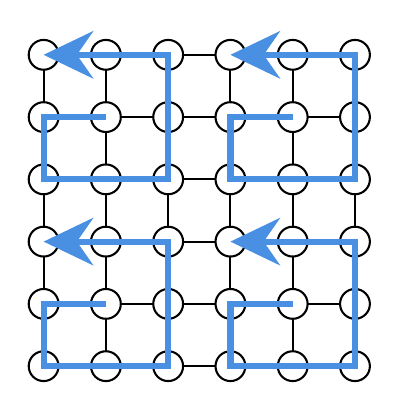
\begin{tikzpicture}[x=0.75pt,y=0.75pt,yscale=-1.5,xscale=1.5]
%uncomment if require: \path (0,301); %set diagram left start at 0, and has height of 301

%Shape: Grid [id:dp04007873776394999] 
\draw  [draw opacity=0][fill={rgb, 255:red, 255; green, 255; blue, 255 }  ,fill opacity=1 ] (280.5,104) -- (380.83,104) -- (380.83,204.33) -- (280.5,204.33) -- cycle ; \draw   (280.5,104) -- (280.5,204.33)(300.5,104) -- (300.5,204.33)(320.5,104) -- (320.5,204.33)(340.5,104) -- (340.5,204.33)(360.5,104) -- (360.5,204.33)(380.5,104) -- (380.5,204.33) ; \draw   (280.5,104) -- (380.83,104)(280.5,124) -- (380.83,124)(280.5,144) -- (380.83,144)(280.5,164) -- (380.83,164)(280.5,184) -- (380.83,184)(280.5,204) -- (380.83,204) ; \draw    ;
%Shape: Circle [id:dp9474225282412638] 
\draw  [fill={rgb, 255:red, 255; green, 255; blue, 255 }  ,fill opacity=1 ] (275.71,184) .. controls (275.71,181.35) and (277.85,179.21) .. (280.5,179.21) .. controls (283.15,179.21) and (285.29,181.35) .. (285.29,184) .. controls (285.29,186.65) and (283.15,188.79) .. (280.5,188.79) .. controls (277.85,188.79) and (275.71,186.65) .. (275.71,184) -- cycle ;
%Shape: Circle [id:dp16610143440847636] 
\draw  [fill={rgb, 255:red, 255; green, 255; blue, 255 }  ,fill opacity=1 ] (295.71,184) .. controls (295.71,181.35) and (297.85,179.21) .. (300.5,179.21) .. controls (303.15,179.21) and (305.29,181.35) .. (305.29,184) .. controls (305.29,186.65) and (303.15,188.79) .. (300.5,188.79) .. controls (297.85,188.79) and (295.71,186.65) .. (295.71,184) -- cycle ;
%Shape: Circle [id:dp03456232735817655] 
\draw  [fill={rgb, 255:red, 255; green, 255; blue, 255 }  ,fill opacity=1 ] (315.71,184) .. controls (315.71,181.35) and (317.85,179.21) .. (320.5,179.21) .. controls (323.15,179.21) and (325.29,181.35) .. (325.29,184) .. controls (325.29,186.65) and (323.15,188.79) .. (320.5,188.79) .. controls (317.85,188.79) and (315.71,186.65) .. (315.71,184) -- cycle ;
%Shape: Circle [id:dp5584249108368513] 
\draw  [fill={rgb, 255:red, 255; green, 255; blue, 255 }  ,fill opacity=1 ] (335.71,184) .. controls (335.71,181.35) and (337.85,179.21) .. (340.5,179.21) .. controls (343.15,179.21) and (345.29,181.35) .. (345.29,184) .. controls (345.29,186.65) and (343.15,188.79) .. (340.5,188.79) .. controls (337.85,188.79) and (335.71,186.65) .. (335.71,184) -- cycle ;
%Shape: Circle [id:dp16243430214118293] 
\draw  [fill={rgb, 255:red, 255; green, 255; blue, 255 }  ,fill opacity=1 ] (355.71,184) .. controls (355.71,181.35) and (357.85,179.21) .. (360.5,179.21) .. controls (363.15,179.21) and (365.29,181.35) .. (365.29,184) .. controls (365.29,186.65) and (363.15,188.79) .. (360.5,188.79) .. controls (357.85,188.79) and (355.71,186.65) .. (355.71,184) -- cycle ;
%Shape: Circle [id:dp16506904974813086] 
\draw  [fill={rgb, 255:red, 255; green, 255; blue, 255 }  ,fill opacity=1 ] (355.71,144) .. controls (355.71,141.35) and (357.85,139.21) .. (360.5,139.21) .. controls (363.15,139.21) and (365.29,141.35) .. (365.29,144) .. controls (365.29,146.65) and (363.15,148.79) .. (360.5,148.79) .. controls (357.85,148.79) and (355.71,146.65) .. (355.71,144) -- cycle ;
%Shape: Circle [id:dp021230581558282724] 
\draw  [fill={rgb, 255:red, 255; green, 255; blue, 255 }  ,fill opacity=1 ] (355.71,164) .. controls (355.71,161.35) and (357.85,159.21) .. (360.5,159.21) .. controls (363.15,159.21) and (365.29,161.35) .. (365.29,164) .. controls (365.29,166.65) and (363.15,168.79) .. (360.5,168.79) .. controls (357.85,168.79) and (355.71,166.65) .. (355.71,164) -- cycle ;
%Shape: Circle [id:dp1804479365808369] 
\draw  [fill={rgb, 255:red, 255; green, 255; blue, 255 }  ,fill opacity=1 ] (335.71,164) .. controls (335.71,161.35) and (337.85,159.21) .. (340.5,159.21) .. controls (343.15,159.21) and (345.29,161.35) .. (345.29,164) .. controls (345.29,166.65) and (343.15,168.79) .. (340.5,168.79) .. controls (337.85,168.79) and (335.71,166.65) .. (335.71,164) -- cycle ;
%Shape: Circle [id:dp47675744505678375] 
\draw  [fill={rgb, 255:red, 255; green, 255; blue, 255 }  ,fill opacity=1 ] (315.71,164) .. controls (315.71,161.35) and (317.85,159.21) .. (320.5,159.21) .. controls (323.15,159.21) and (325.29,161.35) .. (325.29,164) .. controls (325.29,166.65) and (323.15,168.79) .. (320.5,168.79) .. controls (317.85,168.79) and (315.71,166.65) .. (315.71,164) -- cycle ;
%Shape: Circle [id:dp7334743663555192] 
\draw  [fill={rgb, 255:red, 255; green, 255; blue, 255 }  ,fill opacity=1 ] (295.71,164) .. controls (295.71,161.35) and (297.85,159.21) .. (300.5,159.21) .. controls (303.15,159.21) and (305.29,161.35) .. (305.29,164) .. controls (305.29,166.65) and (303.15,168.79) .. (300.5,168.79) .. controls (297.85,168.79) and (295.71,166.65) .. (295.71,164) -- cycle ;
%Shape: Circle [id:dp3042824921088443] 
\draw  [fill={rgb, 255:red, 255; green, 255; blue, 255 }  ,fill opacity=1 ] (275.71,164) .. controls (275.71,161.35) and (277.85,159.21) .. (280.5,159.21) .. controls (283.15,159.21) and (285.29,161.35) .. (285.29,164) .. controls (285.29,166.65) and (283.15,168.79) .. (280.5,168.79) .. controls (277.85,168.79) and (275.71,166.65) .. (275.71,164) -- cycle ;
%Shape: Circle [id:dp15842066644056607] 
\draw  [fill={rgb, 255:red, 255; green, 255; blue, 255 }  ,fill opacity=1 ] (275.71,144) .. controls (275.71,141.35) and (277.85,139.21) .. (280.5,139.21) .. controls (283.15,139.21) and (285.29,141.35) .. (285.29,144) .. controls (285.29,146.65) and (283.15,148.79) .. (280.5,148.79) .. controls (277.85,148.79) and (275.71,146.65) .. (275.71,144) -- cycle ;
%Shape: Circle [id:dp29704787273716904] 
\draw  [fill={rgb, 255:red, 255; green, 255; blue, 255 }  ,fill opacity=1 ] (295.71,144) .. controls (295.71,141.35) and (297.85,139.21) .. (300.5,139.21) .. controls (303.15,139.21) and (305.29,141.35) .. (305.29,144) .. controls (305.29,146.65) and (303.15,148.79) .. (300.5,148.79) .. controls (297.85,148.79) and (295.71,146.65) .. (295.71,144) -- cycle ;
%Shape: Circle [id:dp15622750086846238] 
\draw  [fill={rgb, 255:red, 255; green, 255; blue, 255 }  ,fill opacity=1 ] (315.71,144) .. controls (315.71,141.35) and (317.85,139.21) .. (320.5,139.21) .. controls (323.15,139.21) and (325.29,141.35) .. (325.29,144) .. controls (325.29,146.65) and (323.15,148.79) .. (320.5,148.79) .. controls (317.85,148.79) and (315.71,146.65) .. (315.71,144) -- cycle ;
%Shape: Circle [id:dp8093803696218231] 
\draw  [fill={rgb, 255:red, 255; green, 255; blue, 255 }  ,fill opacity=1 ] (335.71,144) .. controls (335.71,141.35) and (337.85,139.21) .. (340.5,139.21) .. controls (343.15,139.21) and (345.29,141.35) .. (345.29,144) .. controls (345.29,146.65) and (343.15,148.79) .. (340.5,148.79) .. controls (337.85,148.79) and (335.71,146.65) .. (335.71,144) -- cycle ;
%Shape: Circle [id:dp10695862196164163] 
\draw  [fill={rgb, 255:red, 255; green, 255; blue, 255 }  ,fill opacity=1 ] (275.71,124) .. controls (275.71,121.35) and (277.85,119.21) .. (280.5,119.21) .. controls (283.15,119.21) and (285.29,121.35) .. (285.29,124) .. controls (285.29,126.65) and (283.15,128.79) .. (280.5,128.79) .. controls (277.85,128.79) and (275.71,126.65) .. (275.71,124) -- cycle ;
%Shape: Circle [id:dp5260605006362917] 
\draw  [fill={rgb, 255:red, 255; green, 255; blue, 255 }  ,fill opacity=1 ] (295.71,124) .. controls (295.71,121.35) and (297.85,119.21) .. (300.5,119.21) .. controls (303.15,119.21) and (305.29,121.35) .. (305.29,124) .. controls (305.29,126.65) and (303.15,128.79) .. (300.5,128.79) .. controls (297.85,128.79) and (295.71,126.65) .. (295.71,124) -- cycle ;
%Shape: Circle [id:dp8473153436273366] 
\draw  [fill={rgb, 255:red, 255; green, 255; blue, 255 }  ,fill opacity=1 ] (315.71,124) .. controls (315.71,121.35) and (317.85,119.21) .. (320.5,119.21) .. controls (323.15,119.21) and (325.29,121.35) .. (325.29,124) .. controls (325.29,126.65) and (323.15,128.79) .. (320.5,128.79) .. controls (317.85,128.79) and (315.71,126.65) .. (315.71,124) -- cycle ;
%Shape: Circle [id:dp7857758511872395] 
\draw  [fill={rgb, 255:red, 255; green, 255; blue, 255 }  ,fill opacity=1 ] (335.71,124) .. controls (335.71,121.35) and (337.85,119.21) .. (340.5,119.21) .. controls (343.15,119.21) and (345.29,121.35) .. (345.29,124) .. controls (345.29,126.65) and (343.15,128.79) .. (340.5,128.79) .. controls (337.85,128.79) and (335.71,126.65) .. (335.71,124) -- cycle ;
%Shape: Circle [id:dp3662097810280891] 
\draw  [fill={rgb, 255:red, 255; green, 255; blue, 255 }  ,fill opacity=1 ] (355.71,124) .. controls (355.71,121.35) and (357.85,119.21) .. (360.5,119.21) .. controls (363.15,119.21) and (365.29,121.35) .. (365.29,124) .. controls (365.29,126.65) and (363.15,128.79) .. (360.5,128.79) .. controls (357.85,128.79) and (355.71,126.65) .. (355.71,124) -- cycle ;
%Shape: Circle [id:dp05943436716946482] 
\draw  [fill={rgb, 255:red, 255; green, 255; blue, 255 }  ,fill opacity=1 ] (275.71,104) .. controls (275.71,101.35) and (277.85,99.21) .. (280.5,99.21) .. controls (283.15,99.21) and (285.29,101.35) .. (285.29,104) .. controls (285.29,106.65) and (283.15,108.79) .. (280.5,108.79) .. controls (277.85,108.79) and (275.71,106.65) .. (275.71,104) -- cycle ;
%Shape: Circle [id:dp809722377804333] 
\draw  [fill={rgb, 255:red, 255; green, 255; blue, 255 }  ,fill opacity=1 ] (295.71,104) .. controls (295.71,101.35) and (297.85,99.21) .. (300.5,99.21) .. controls (303.15,99.21) and (305.29,101.35) .. (305.29,104) .. controls (305.29,106.65) and (303.15,108.79) .. (300.5,108.79) .. controls (297.85,108.79) and (295.71,106.65) .. (295.71,104) -- cycle ;
%Shape: Circle [id:dp2456656687962917] 
\draw  [fill={rgb, 255:red, 255; green, 255; blue, 255 }  ,fill opacity=1 ] (315.71,104) .. controls (315.71,101.35) and (317.85,99.21) .. (320.5,99.21) .. controls (323.15,99.21) and (325.29,101.35) .. (325.29,104) .. controls (325.29,106.65) and (323.15,108.79) .. (320.5,108.79) .. controls (317.85,108.79) and (315.71,106.65) .. (315.71,104) -- cycle ;
%Shape: Circle [id:dp4412509805400553] 
\draw  [fill={rgb, 255:red, 255; green, 255; blue, 255 }  ,fill opacity=1 ] (335.71,104) .. controls (335.71,101.35) and (337.85,99.21) .. (340.5,99.21) .. controls (343.15,99.21) and (345.29,101.35) .. (345.29,104) .. controls (345.29,106.65) and (343.15,108.79) .. (340.5,108.79) .. controls (337.85,108.79) and (335.71,106.65) .. (335.71,104) -- cycle ;
%Shape: Circle [id:dp9250884814038944] 
\draw  [fill={rgb, 255:red, 255; green, 255; blue, 255 }  ,fill opacity=1 ] (355.71,104) .. controls (355.71,101.35) and (357.85,99.21) .. (360.5,99.21) .. controls (363.15,99.21) and (365.29,101.35) .. (365.29,104) .. controls (365.29,106.65) and (363.15,108.79) .. (360.5,108.79) .. controls (357.85,108.79) and (355.71,106.65) .. (355.71,104) -- cycle ;
%Shape: Circle [id:dp5750759061407391] 
\draw  [fill={rgb, 255:red, 255; green, 255; blue, 255 }  ,fill opacity=1 ] (375.71,104) .. controls (375.71,101.35) and (377.85,99.21) .. (380.5,99.21) .. controls (383.15,99.21) and (385.29,101.35) .. (385.29,104) .. controls (385.29,106.65) and (383.15,108.79) .. (380.5,108.79) .. controls (377.85,108.79) and (375.71,106.65) .. (375.71,104) -- cycle ;
%Shape: Circle [id:dp31417490416250016] 
\draw  [fill={rgb, 255:red, 255; green, 255; blue, 255 }  ,fill opacity=1 ] (375.71,124) .. controls (375.71,121.35) and (377.85,119.21) .. (380.5,119.21) .. controls (383.15,119.21) and (385.29,121.35) .. (385.29,124) .. controls (385.29,126.65) and (383.15,128.79) .. (380.5,128.79) .. controls (377.85,128.79) and (375.71,126.65) .. (375.71,124) -- cycle ;
%Shape: Circle [id:dp006667999859743423] 
\draw  [fill={rgb, 255:red, 255; green, 255; blue, 255 }  ,fill opacity=1 ] (375.71,144) .. controls (375.71,141.35) and (377.85,139.21) .. (380.5,139.21) .. controls (383.15,139.21) and (385.29,141.35) .. (385.29,144) .. controls (385.29,146.65) and (383.15,148.79) .. (380.5,148.79) .. controls (377.85,148.79) and (375.71,146.65) .. (375.71,144) -- cycle ;
%Shape: Circle [id:dp12634282620893122] 
\draw  [fill={rgb, 255:red, 255; green, 255; blue, 255 }  ,fill opacity=1 ] (375.71,164) .. controls (375.71,161.35) and (377.85,159.21) .. (380.5,159.21) .. controls (383.15,159.21) and (385.29,161.35) .. (385.29,164) .. controls (385.29,166.65) and (383.15,168.79) .. (380.5,168.79) .. controls (377.85,168.79) and (375.71,166.65) .. (375.71,164) -- cycle ;
%Shape: Circle [id:dp19045978877802572] 
\draw  [fill={rgb, 255:red, 255; green, 255; blue, 255 }  ,fill opacity=1 ] (275.71,204) .. controls (275.71,201.35) and (277.85,199.21) .. (280.5,199.21) .. controls (283.15,199.21) and (285.29,201.35) .. (285.29,204) .. controls (285.29,206.65) and (283.15,208.79) .. (280.5,208.79) .. controls (277.85,208.79) and (275.71,206.65) .. (275.71,204) -- cycle ;
%Shape: Circle [id:dp8417560897443137] 
\draw  [fill={rgb, 255:red, 255; green, 255; blue, 255 }  ,fill opacity=1 ] (295.71,204) .. controls (295.71,201.35) and (297.85,199.21) .. (300.5,199.21) .. controls (303.15,199.21) and (305.29,201.35) .. (305.29,204) .. controls (305.29,206.65) and (303.15,208.79) .. (300.5,208.79) .. controls (297.85,208.79) and (295.71,206.65) .. (295.71,204) -- cycle ;
%Shape: Circle [id:dp36466854494079004] 
\draw  [fill={rgb, 255:red, 255; green, 255; blue, 255 }  ,fill opacity=1 ] (315.71,204) .. controls (315.71,201.35) and (317.85,199.21) .. (320.5,199.21) .. controls (323.15,199.21) and (325.29,201.35) .. (325.29,204) .. controls (325.29,206.65) and (323.15,208.79) .. (320.5,208.79) .. controls (317.85,208.79) and (315.71,206.65) .. (315.71,204) -- cycle ;
%Shape: Circle [id:dp08813117271342974] 
\draw  [fill={rgb, 255:red, 255; green, 255; blue, 255 }  ,fill opacity=1 ] (335.71,204) .. controls (335.71,201.35) and (337.85,199.21) .. (340.5,199.21) .. controls (343.15,199.21) and (345.29,201.35) .. (345.29,204) .. controls (345.29,206.65) and (343.15,208.79) .. (340.5,208.79) .. controls (337.85,208.79) and (335.71,206.65) .. (335.71,204) -- cycle ;
%Shape: Circle [id:dp12510148076826888] 
\draw  [fill={rgb, 255:red, 255; green, 255; blue, 255 }  ,fill opacity=1 ] (355.71,204) .. controls (355.71,201.35) and (357.85,199.21) .. (360.5,199.21) .. controls (363.15,199.21) and (365.29,201.35) .. (365.29,204) .. controls (365.29,206.65) and (363.15,208.79) .. (360.5,208.79) .. controls (357.85,208.79) and (355.71,206.65) .. (355.71,204) -- cycle ;
%Shape: Circle [id:dp32302714489826934] 
\draw  [fill={rgb, 255:red, 255; green, 255; blue, 255 }  ,fill opacity=1 ] (375.71,204) .. controls (375.71,201.35) and (377.85,199.21) .. (380.5,199.21) .. controls (383.15,199.21) and (385.29,201.35) .. (385.29,204) .. controls (385.29,206.65) and (383.15,208.79) .. (380.5,208.79) .. controls (377.85,208.79) and (375.71,206.65) .. (375.71,204) -- cycle ;
%Shape: Circle [id:dp047477242771539085] 
\draw  [fill={rgb, 255:red, 255; green, 255; blue, 255 }  ,fill opacity=1 ] (375.71,184) .. controls (375.71,181.35) and (377.85,179.21) .. (380.5,179.21) .. controls (383.15,179.21) and (385.29,181.35) .. (385.29,184) .. controls (385.29,186.65) and (383.15,188.79) .. (380.5,188.79) .. controls (377.85,188.79) and (375.71,186.65) .. (375.71,184) -- cycle ;
%Straight Lines [id:da9724777887310767] 
\draw [color={rgb, 255:red, 74; green, 144; blue, 226 }  ,draw opacity=1 ][line width=2.25]    (300.5,124) -- (280.5,124) -- (280.5,144) -- (320.5,144) -- (320.5,104) -- (284.5,104) ;
\draw [shift={(280.5,104)}, rotate = 360] [fill={rgb, 255:red, 74; green, 144; blue, 226 }  ,fill opacity=1 ][line width=2.25]  [draw opacity=0] (16.07,-7.72) -- (0,0) -- (16.07,7.72) -- (10.67,0) -- cycle    ;

%Straight Lines [id:da17976314984393982] 
\draw [color={rgb, 255:red, 74; green, 144; blue, 226 }  ,draw opacity=1 ][line width=2.25]    (360.5,124) -- (340.5,124) -- (340.5,144) -- (380.5,144) -- (380.5,104) -- (344.5,104) ;
\draw [shift={(340.5,104)}, rotate = 360] [fill={rgb, 255:red, 74; green, 144; blue, 226 }  ,fill opacity=1 ][line width=2.25]  [draw opacity=0] (16.07,-7.72) -- (0,0) -- (16.07,7.72) -- (10.67,0) -- cycle    ;

%Straight Lines [id:da7541239074637796] 
\draw [color={rgb, 255:red, 74; green, 144; blue, 226 }  ,draw opacity=1 ][line width=2.25]    (300.5,184) -- (280.5,184) -- (280.5,204) -- (320.5,204) -- (320.5,164) -- (284.5,164) ;
\draw [shift={(280.5,164)}, rotate = 360] [fill={rgb, 255:red, 74; green, 144; blue, 226 }  ,fill opacity=1 ][line width=2.25]  [draw opacity=0] (16.07,-7.72) -- (0,0) -- (16.07,7.72) -- (10.67,0) -- cycle    ;

%Straight Lines [id:da7981579653949769] 
\draw [color={rgb, 255:red, 74; green, 144; blue, 226 }  ,draw opacity=1 ][line width=2.25]    (360.5,184) -- (340.5,184) -- (340.5,204) -- (380.5,204) -- (380.5,164) -- (344.5,164) ;
\draw [shift={(340.5,164)}, rotate = 360] [fill={rgb, 255:red, 74; green, 144; blue, 226 }  ,fill opacity=1 ][line width=2.25]  [draw opacity=0] (16.07,-7.72) -- (0,0) -- (16.07,7.72) -- (10.67,0) -- cycle    ;





\end{tikzpicture}

			\end{center}
			\caption{Cache-aware ordering, enumeration along the arrow lines}
			\label{fig:cacheorder}
		\end{figure}
		
		This ordering scheme utilizes the fact, that data which is "located in a neighbourhood in memory respectively" can be accessed much quicker and thus fastens the operations used on the matrices.

	\item Wave front orderings (diagonal ordering)

		\begin{figure}[ht!]
			\begin{center}
				

\tikzset{every picture/.style={line width=0.75pt}} %set default line width to 0.75pt        

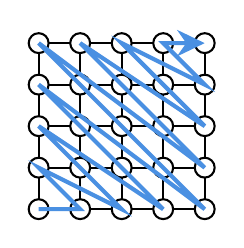
\begin{tikzpicture}[x=0.75pt,y=0.75pt,yscale=-1,xscale=1]
%uncomment if require: \path (0,260); %set diagram left start at 0, and has height of 260

%Shape: Grid [id:dp23256726802759253] 
\draw  [draw opacity=0][fill={rgb, 255:red, 255; green, 255; blue, 255 }  ,fill opacity=1 ] (290.5,90) -- (370.67,90) -- (370.67,170.5) -- (290.5,170.5) -- cycle ; \draw   (290.5,90) -- (290.5,170.5)(310.5,90) -- (310.5,170.5)(330.5,90) -- (330.5,170.5)(350.5,90) -- (350.5,170.5)(370.5,90) -- (370.5,170.5) ; \draw   (290.5,90) -- (370.67,90)(290.5,110) -- (370.67,110)(290.5,130) -- (370.67,130)(290.5,150) -- (370.67,150)(290.5,170) -- (370.67,170) ; \draw    ;
%Shape: Circle [id:dp8205642245940685] 
\draw  [fill={rgb, 255:red, 255; green, 255; blue, 255 }  ,fill opacity=1 ] (285.71,170) .. controls (285.71,167.35) and (287.85,165.21) .. (290.5,165.21) .. controls (293.15,165.21) and (295.29,167.35) .. (295.29,170) .. controls (295.29,172.65) and (293.15,174.79) .. (290.5,174.79) .. controls (287.85,174.79) and (285.71,172.65) .. (285.71,170) -- cycle ;
%Shape: Circle [id:dp366405571034746] 
\draw  [fill={rgb, 255:red, 255; green, 255; blue, 255 }  ,fill opacity=1 ] (305.71,170) .. controls (305.71,167.35) and (307.85,165.21) .. (310.5,165.21) .. controls (313.15,165.21) and (315.29,167.35) .. (315.29,170) .. controls (315.29,172.65) and (313.15,174.79) .. (310.5,174.79) .. controls (307.85,174.79) and (305.71,172.65) .. (305.71,170) -- cycle ;
%Shape: Circle [id:dp15906627820442676] 
\draw  [fill={rgb, 255:red, 255; green, 255; blue, 255 }  ,fill opacity=1 ] (325.71,170) .. controls (325.71,167.35) and (327.85,165.21) .. (330.5,165.21) .. controls (333.15,165.21) and (335.29,167.35) .. (335.29,170) .. controls (335.29,172.65) and (333.15,174.79) .. (330.5,174.79) .. controls (327.85,174.79) and (325.71,172.65) .. (325.71,170) -- cycle ;
%Shape: Circle [id:dp40387678987476283] 
\draw  [fill={rgb, 255:red, 255; green, 255; blue, 255 }  ,fill opacity=1 ] (345.71,170) .. controls (345.71,167.35) and (347.85,165.21) .. (350.5,165.21) .. controls (353.15,165.21) and (355.29,167.35) .. (355.29,170) .. controls (355.29,172.65) and (353.15,174.79) .. (350.5,174.79) .. controls (347.85,174.79) and (345.71,172.65) .. (345.71,170) -- cycle ;
%Shape: Circle [id:dp004033840648062892] 
\draw  [fill={rgb, 255:red, 255; green, 255; blue, 255 }  ,fill opacity=1 ] (365.71,170) .. controls (365.71,167.35) and (367.85,165.21) .. (370.5,165.21) .. controls (373.15,165.21) and (375.29,167.35) .. (375.29,170) .. controls (375.29,172.65) and (373.15,174.79) .. (370.5,174.79) .. controls (367.85,174.79) and (365.71,172.65) .. (365.71,170) -- cycle ;
%Shape: Circle [id:dp7856406790445534] 
\draw  [fill={rgb, 255:red, 255; green, 255; blue, 255 }  ,fill opacity=1 ] (365.71,130) .. controls (365.71,127.35) and (367.85,125.21) .. (370.5,125.21) .. controls (373.15,125.21) and (375.29,127.35) .. (375.29,130) .. controls (375.29,132.65) and (373.15,134.79) .. (370.5,134.79) .. controls (367.85,134.79) and (365.71,132.65) .. (365.71,130) -- cycle ;
%Shape: Circle [id:dp9423249034074639] 
\draw  [fill={rgb, 255:red, 255; green, 255; blue, 255 }  ,fill opacity=1 ] (365.71,150) .. controls (365.71,147.35) and (367.85,145.21) .. (370.5,145.21) .. controls (373.15,145.21) and (375.29,147.35) .. (375.29,150) .. controls (375.29,152.65) and (373.15,154.79) .. (370.5,154.79) .. controls (367.85,154.79) and (365.71,152.65) .. (365.71,150) -- cycle ;
%Shape: Circle [id:dp4603048926021358] 
\draw  [fill={rgb, 255:red, 255; green, 255; blue, 255 }  ,fill opacity=1 ] (345.71,150) .. controls (345.71,147.35) and (347.85,145.21) .. (350.5,145.21) .. controls (353.15,145.21) and (355.29,147.35) .. (355.29,150) .. controls (355.29,152.65) and (353.15,154.79) .. (350.5,154.79) .. controls (347.85,154.79) and (345.71,152.65) .. (345.71,150) -- cycle ;
%Shape: Circle [id:dp3221609399549774] 
\draw  [fill={rgb, 255:red, 255; green, 255; blue, 255 }  ,fill opacity=1 ] (325.71,150) .. controls (325.71,147.35) and (327.85,145.21) .. (330.5,145.21) .. controls (333.15,145.21) and (335.29,147.35) .. (335.29,150) .. controls (335.29,152.65) and (333.15,154.79) .. (330.5,154.79) .. controls (327.85,154.79) and (325.71,152.65) .. (325.71,150) -- cycle ;
%Shape: Circle [id:dp2913063050312137] 
\draw  [fill={rgb, 255:red, 255; green, 255; blue, 255 }  ,fill opacity=1 ] (305.71,150) .. controls (305.71,147.35) and (307.85,145.21) .. (310.5,145.21) .. controls (313.15,145.21) and (315.29,147.35) .. (315.29,150) .. controls (315.29,152.65) and (313.15,154.79) .. (310.5,154.79) .. controls (307.85,154.79) and (305.71,152.65) .. (305.71,150) -- cycle ;
%Shape: Circle [id:dp08553242219473445] 
\draw  [fill={rgb, 255:red, 255; green, 255; blue, 255 }  ,fill opacity=1 ] (285.71,150) .. controls (285.71,147.35) and (287.85,145.21) .. (290.5,145.21) .. controls (293.15,145.21) and (295.29,147.35) .. (295.29,150) .. controls (295.29,152.65) and (293.15,154.79) .. (290.5,154.79) .. controls (287.85,154.79) and (285.71,152.65) .. (285.71,150) -- cycle ;
%Shape: Circle [id:dp9457745167457556] 
\draw  [fill={rgb, 255:red, 255; green, 255; blue, 255 }  ,fill opacity=1 ] (285.71,130) .. controls (285.71,127.35) and (287.85,125.21) .. (290.5,125.21) .. controls (293.15,125.21) and (295.29,127.35) .. (295.29,130) .. controls (295.29,132.65) and (293.15,134.79) .. (290.5,134.79) .. controls (287.85,134.79) and (285.71,132.65) .. (285.71,130) -- cycle ;
%Shape: Circle [id:dp060234058910684674] 
\draw  [fill={rgb, 255:red, 255; green, 255; blue, 255 }  ,fill opacity=1 ] (305.71,130) .. controls (305.71,127.35) and (307.85,125.21) .. (310.5,125.21) .. controls (313.15,125.21) and (315.29,127.35) .. (315.29,130) .. controls (315.29,132.65) and (313.15,134.79) .. (310.5,134.79) .. controls (307.85,134.79) and (305.71,132.65) .. (305.71,130) -- cycle ;
%Shape: Circle [id:dp9752050660650597] 
\draw  [fill={rgb, 255:red, 255; green, 255; blue, 255 }  ,fill opacity=1 ] (325.71,130) .. controls (325.71,127.35) and (327.85,125.21) .. (330.5,125.21) .. controls (333.15,125.21) and (335.29,127.35) .. (335.29,130) .. controls (335.29,132.65) and (333.15,134.79) .. (330.5,134.79) .. controls (327.85,134.79) and (325.71,132.65) .. (325.71,130) -- cycle ;
%Shape: Circle [id:dp2719113469792509] 
\draw  [fill={rgb, 255:red, 255; green, 255; blue, 255 }  ,fill opacity=1 ] (345.71,130) .. controls (345.71,127.35) and (347.85,125.21) .. (350.5,125.21) .. controls (353.15,125.21) and (355.29,127.35) .. (355.29,130) .. controls (355.29,132.65) and (353.15,134.79) .. (350.5,134.79) .. controls (347.85,134.79) and (345.71,132.65) .. (345.71,130) -- cycle ;
%Shape: Circle [id:dp327036969138353] 
\draw  [fill={rgb, 255:red, 255; green, 255; blue, 255 }  ,fill opacity=1 ] (285.71,110) .. controls (285.71,107.35) and (287.85,105.21) .. (290.5,105.21) .. controls (293.15,105.21) and (295.29,107.35) .. (295.29,110) .. controls (295.29,112.65) and (293.15,114.79) .. (290.5,114.79) .. controls (287.85,114.79) and (285.71,112.65) .. (285.71,110) -- cycle ;
%Shape: Circle [id:dp8914806778108353] 
\draw  [fill={rgb, 255:red, 255; green, 255; blue, 255 }  ,fill opacity=1 ] (305.71,110) .. controls (305.71,107.35) and (307.85,105.21) .. (310.5,105.21) .. controls (313.15,105.21) and (315.29,107.35) .. (315.29,110) .. controls (315.29,112.65) and (313.15,114.79) .. (310.5,114.79) .. controls (307.85,114.79) and (305.71,112.65) .. (305.71,110) -- cycle ;
%Shape: Circle [id:dp3227047795012228] 
\draw  [fill={rgb, 255:red, 255; green, 255; blue, 255 }  ,fill opacity=1 ] (325.71,110) .. controls (325.71,107.35) and (327.85,105.21) .. (330.5,105.21) .. controls (333.15,105.21) and (335.29,107.35) .. (335.29,110) .. controls (335.29,112.65) and (333.15,114.79) .. (330.5,114.79) .. controls (327.85,114.79) and (325.71,112.65) .. (325.71,110) -- cycle ;
%Shape: Circle [id:dp29660618179137943] 
\draw  [fill={rgb, 255:red, 255; green, 255; blue, 255 }  ,fill opacity=1 ] (345.71,110) .. controls (345.71,107.35) and (347.85,105.21) .. (350.5,105.21) .. controls (353.15,105.21) and (355.29,107.35) .. (355.29,110) .. controls (355.29,112.65) and (353.15,114.79) .. (350.5,114.79) .. controls (347.85,114.79) and (345.71,112.65) .. (345.71,110) -- cycle ;
%Shape: Circle [id:dp399216711175046] 
\draw  [fill={rgb, 255:red, 255; green, 255; blue, 255 }  ,fill opacity=1 ] (365.71,110) .. controls (365.71,107.35) and (367.85,105.21) .. (370.5,105.21) .. controls (373.15,105.21) and (375.29,107.35) .. (375.29,110) .. controls (375.29,112.65) and (373.15,114.79) .. (370.5,114.79) .. controls (367.85,114.79) and (365.71,112.65) .. (365.71,110) -- cycle ;
%Shape: Circle [id:dp7712238918530412] 
\draw  [fill={rgb, 255:red, 255; green, 255; blue, 255 }  ,fill opacity=1 ] (285.71,90) .. controls (285.71,87.35) and (287.85,85.21) .. (290.5,85.21) .. controls (293.15,85.21) and (295.29,87.35) .. (295.29,90) .. controls (295.29,92.65) and (293.15,94.79) .. (290.5,94.79) .. controls (287.85,94.79) and (285.71,92.65) .. (285.71,90) -- cycle ;
%Shape: Circle [id:dp03381617924152547] 
\draw  [fill={rgb, 255:red, 255; green, 255; blue, 255 }  ,fill opacity=1 ] (305.71,90) .. controls (305.71,87.35) and (307.85,85.21) .. (310.5,85.21) .. controls (313.15,85.21) and (315.29,87.35) .. (315.29,90) .. controls (315.29,92.65) and (313.15,94.79) .. (310.5,94.79) .. controls (307.85,94.79) and (305.71,92.65) .. (305.71,90) -- cycle ;
%Shape: Circle [id:dp21486580128810973] 
\draw  [fill={rgb, 255:red, 255; green, 255; blue, 255 }  ,fill opacity=1 ] (325.71,90) .. controls (325.71,87.35) and (327.85,85.21) .. (330.5,85.21) .. controls (333.15,85.21) and (335.29,87.35) .. (335.29,90) .. controls (335.29,92.65) and (333.15,94.79) .. (330.5,94.79) .. controls (327.85,94.79) and (325.71,92.65) .. (325.71,90) -- cycle ;
%Shape: Circle [id:dp7779334748918709] 
\draw  [fill={rgb, 255:red, 255; green, 255; blue, 255 }  ,fill opacity=1 ] (345.71,90) .. controls (345.71,87.35) and (347.85,85.21) .. (350.5,85.21) .. controls (353.15,85.21) and (355.29,87.35) .. (355.29,90) .. controls (355.29,92.65) and (353.15,94.79) .. (350.5,94.79) .. controls (347.85,94.79) and (345.71,92.65) .. (345.71,90) -- cycle ;
%Shape: Circle [id:dp8817520223622921] 
\draw  [fill={rgb, 255:red, 255; green, 255; blue, 255 }  ,fill opacity=1 ] (365.71,90) .. controls (365.71,87.35) and (367.85,85.21) .. (370.5,85.21) .. controls (373.15,85.21) and (375.29,87.35) .. (375.29,90) .. controls (375.29,92.65) and (373.15,94.79) .. (370.5,94.79) .. controls (367.85,94.79) and (365.71,92.65) .. (365.71,90) -- cycle ;
%Straight Lines [id:da9184012573250542] 
\draw [color={rgb, 255:red, 74; green, 144; blue, 226 }  ,draw opacity=1 ][line width=1.5]    (290.5,170) -- (310.5,170) -- (290.5,150) -- (330.5,170) -- (290.5,130) -- (350.5,170) -- (290.5,110) -- (370.5,170) -- (290.5,90) -- (370.5,150) -- (310.5,90) -- (370.5,130) -- (330.5,90) -- (370.5,110) -- (350.5,90) -- (367.5,90) ;
\draw [shift={(370.5,90)}, rotate = 180] [fill={rgb, 255:red, 74; green, 144; blue, 226 }  ,fill opacity=1 ][line width=1.5]  [draw opacity=0] (13.4,-6.43) -- (0,0) -- (13.4,6.44) -- (8.9,0) -- cycle    ;





\end{tikzpicture}
			\end{center}
			\caption{Wave front ordering, enumeration along the arrow lines}
			\label{fig:waveorder}
		\end{figure}
		
\end{enumerate}

\section{Assembling}%
\label{sec:Assembling}

For the Poisson equation
\[
-\laplace u = f
.\] 
we can assemble a linear system $Au=f$ by applying the discrete operator $\laplace_{h}^{(5)}$ instead of $\laplace$ and by evaluating in the grid nodes
\[
	\begin{array}{ccl}
	A = (a_{rs}) 
	\quad&\text{ with }\quad 
	&a_{r(i,j),s(i',j')}= \frac{1}{h^{2}}\begin{cases}
		4 &\text{,if } r=s \\
		-1 &\text{,if } \abs{i-i'} = 1 \text{ and } \abs{j-j'} = 0 \\
		-1 &\text{,if } \abs{i-i'} = 0 \text{ and } \abs{j-j'} = 1 \\
		0 &\text{,otherwise}
	\end{cases} \\ \\
	f = (f_{r}) 
	\quad&\text{ with }\quad
	&f_{r(i,j)}=f(ih, jh)=f(x_{i}, y_{i})
	\end{array}
\] 
\[
	 A \stackeq{\wedge} -\laplace_{h}^{(5)}
.\] 

\section{Boundary conditions}%
\label{sec:Boundary condition}
For Dirichlet boundary condition the value $u$ at boundary nodes is fixed.

A node is boundary node if
\[
i \in  \{0, N_{x}+1\} \quad\text{ or }\quad j \in  \{0,N_{y}+1\}
.\] 

And so $u_{i,j} = g_{i,j}$ if $(i,j)$ is a boundary node.

The boundary condition can be realized by eliminating rows/columns in the matrix, i.e. let $r=l(i,j)$ a boundary index

\begin{align*}
	f &\leftarrow f-A_{\ast,r}\cdot g_{i,j} \\
	A_{r,\ast} &\leftarrow \delta_{r,s} \\
	A_{*,r} &\leftarrow \delta_{r,s} \\
	f_{r} &\leftarrow g_{i,j}
\end{align*}

\[
A\cdot \underline{u} = \underline{f}  
.\] 
\[
A = \begin{pmatrix}
	X & 
	\begin{matrix}
		0 \\
		\vdots
	\end{matrix} & X \\
	\begin{matrix}
		0 & \cdots 
	\end{matrix} & 1 &
	\begin{matrix}
		 \cdots & 0
	\end{matrix}\\
	X & \begin{matrix}
	\vdots \\
	0
	\end{matrix}
	  & X
	
	\end{pmatrix}
.\] 

\section{Structure of the matrix}%
\label{sec:Structure of the matrix}
(before eliminating the boundary conditions)
\begin{enumerate}[label=\alph{enumi})]
	\item Lexicographical ordering
		\[
		A= \frac{1}{h^{2}}
		\underbrace{
		\begin{bmatrix}
			[A_{0}] & [-I] &&& \\
			[-I] & [A_0] &&&\\
				 &&\ddots && \\
				 &&& [A_0] & [-I] \\
				 &&& [-I]& [A_0]
		\end{bmatrix}
		}_{N_{x}+2 \text{ blocks}}
		.\] 

		\[
		A_0 = \begin{bmatrix}
			4 & -1 &&& \\
			-1 & 4 & -1 && \\
			 & -1 & \ddots && \\
			 &&&\ddots & -1 \\
			 &&&-1 & 4
		\end{bmatrix}
		.\] 
	\item Red-Black ordering

		\[
			\begin{bmatrix}
				D_{r} & B \\
				B^{T} & D_{b}
			\end{bmatrix}
			\quad \text{with}\quad D_{r/b}=-\frac{1}{h^{2}}I_{r/b}
		.\] 
		B contains the values from the coupling of the nodes
\end{enumerate}

Variation of the PDE:
\[
\partial_{t}u- \laplace u=f
.\] 
Simple backward Euler scheme for $\partial_{t}$
\[
\frac{1}{\tau}u^{m+1}- \laplace u^{m+1} = f -\frac{1}{\tau}u^{m}
.\] 
with $u^{m} \equiv u(t^{m})$ with $0=t^{0}<t^{1}< \ldots  < t^{md}$ and $\tau:=t^{m+1}-t^{m}$.

The corresponding FD discretization reads:

\[
	\left(\frac{1}{\tau}I + A\right) u^{m+1} = f + \frac{1}{\tau}u^{m}
.\] 

\section{Properties of the linear system}%
\label{sec:Properties of the linear system}

\begin{definition}
\label{thm:typeOfMatrices}
	A matrix $A \in  \R^{n \times n}$ is called
	\begin{itemize}
		\item \underline{Z-matrix}, if $a_{ij}\leq 0\quad \forall i\neq j$
		\item \underline{symmetric positive definite}, if $A=A^{T}$ and $A>0$, i.e. $u^{T}Au>0\quad\forall u \in \R^{n} \setminus 0$
		\item \underline{positive definite} , if $A+A^{T}>0$
		\item \underline{M-matrix}, if $A$ is Z-matrix and $\Re(\lambda) > 0 \quad\forall \lambda \in \sigma (A)$
		\item \underline{M$_{0}$-Matrix}, if it is pos. def. and Z-matrix (M$_{0}$-matrix is an M-matrix)
	\end{itemize}
\end{definition}

\begin{definition}
\label{thm:adjacenyGraph}
Let $A$ be a (sparse) matrix. The graph $G_{A}=(V,E)$ with $E \subset V \times V$ is called \underline{adjacency graph} of $A$ if 
\begin{itemize}[label=]
	\item $V$ represents the $n$ unknowns/rows/columns
	\item $V=\{1, \ldots, n\}$
	\item $E=\{(i,j) \in  V \times V : a_{ij}\neq 0\}$
\end{itemize}
(The edges represent the relation: equations $i$ involves unknown $j$)
\end{definition}

\begin{definition}
\label{thm:irreducible}
A matrix $A$ is called \underline{irreducible} if for $G_{A}=(V,E)$:
\[
	\forall i,j \in V ~:~ \exists \text{ sequence of edges } (e_0, e_1, \ldots , e_{n}) \subset E
\] 
such that
\[
	e_0=(i, k_0), e_1=(k_0,k_1),\ldots , e_{m}=(k_{m-1},j) \quad \text{with } k_{j} \in V
.\] 

(All vertices are connected by a sequence of edges)
\[
	\mathcal{IR}:= \{A \in  \R^{n \times  n} | A \text{ is irreducible}\}
.\] 
\end{definition}

\begin{definition}
\label{thm:WDDmatrices}
\begin{align*}
	WDD:= &\left\{ A \in \R^{n \times n}, \abs{a_{j,j}}  \geq \sum_{i\neq j}^{}{\abs{a_{i,j}} } \quad \forall j \right\}  \\
		 = &\left\{ A \in R^{n \times }, \abs{a_{i,i}} \geq \sum_{i\neq j}^{}{\abs{a_{i,j}} } \quad \forall i \right\} 
\end{align*}
are the weakly diagonal dominant matrices.
\[
DD:= \left\{ A \in WDD, \exists j : ">" \right\} 
\] 
are diagonal dominant matrices.
\[
SDD := \left\{ A \in WDD, \forall j : ">" \right\} 
\] 
are the strictly diagonal dominant matrices.
\[
IDD := \left\{ A \in DD, A \text{ is irreducible} \right\} 
\] 
are the irreducible diagonal dominant matrices.
\end{definition}

\begin{theorem}(Gershgorin)
\label{thm:gershgorin}
Any eigenvalue $\lambda \in \sigma (A)$ is located in one of the closed discs in the complex plane centered at $a_{i,i}$ and having the radius
\[
	\rho_{i} = \sum_{\substack{j=0 \\ j \neq i}}^{n}{\abs{a_{i,j}} }
.\] 
In other words : 
\[
	\forall \lambda \in \sigma (A) \exists i \text{ such that } \abs{\lambda - a_{i,i}}  \leq \sum_{\substack{j=0 \\ j \neq i}}^{n}{\abs{a_{i,j}} }
.\] 
\end{theorem}

\begin{proof}
\label{thm:gershgorinproof}
	Let $x$ be an eigenvector associated to eigenvalue $\lambda$ and let $m$ be the index of the component with largest modulus in $x$.

	Scale $x$, s.t.
	\[
	\abs{x_{m}}  = 1 \text{ and } \abs{x_{i}} \leq 1 \quad \forall i \neq m
	.\] 
	Since $x$ is an eigenvector to $A$, we have
	\[
		(\lambda - a_{n,m}) x_{m} = - \sum_{\substack{j=1 \\ j \neq m}}^{n}{\abs{a_{m,j}} x_{j}}
	.\] 
	Taking the absolute value of this, we get
	\[
		\abs{\lambda - a_{m,m}}  \leq \sum_{j\neq m}^{}{\abs{a_{m,j}} \abs{x_{j}} } \leq \sum_{j\neq m}^{}{\abs{a_{m,j}} } = \rho_{m}
	.\] 
\end{proof}
\begin{figure}[H]
	\center
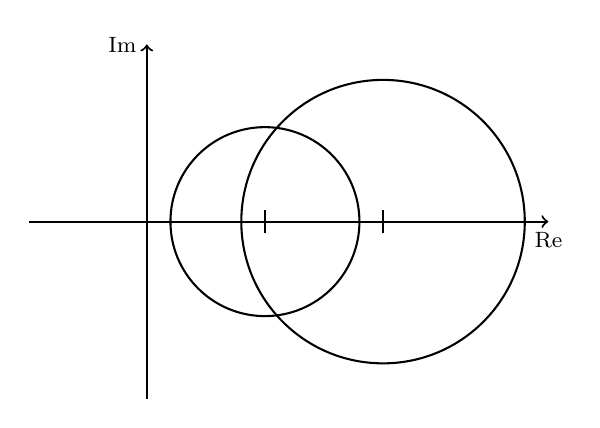
\begin{tikzpicture}[scale=3]
		
		\def \xone{0};
		\def \yone{0};		
		% draw coordinate system
		\coordinate (A) at (\xone,\yone);
		
		\draw[->] (A) ++ (0,-0.75) -- ++(0,1.5);
		\draw[->] (A) ++ (-0.5,0)-- ++(2.2,0);

		% a circle is easier to draw than another object
        \draw (A) ++(0.5,0) circle (0.4cm);
		\draw (A) ++(0.5,-0.05) -- ++(0,0.1);
        \draw (A) ++(1,0) circle (0.6cm);
		\draw (A) ++(1,-0.05) -- ++(0,0.1);

        \fill[black,font=\footnotesize] (A) ++(1.7,0) node[below] {Re}
										(A) ++(0,0.75) node[left] {Im};
                                        
\end{tikzpicture}

\caption{Example for Gershgorin discs}
\label{gerschgorin_discs}
\end{figure}

\begin{theorem}
\label{thm:gershgorinboundary}
	Let $A$ be irreducible and assume that an eigenvalue $\lambda$ lies on the boundary of the union of all Gershgorin discs. Then $\lambda$ lies on the boundary of all Gershgorin discs.
\end{theorem}

\begin{proof}
\label{thm:gershgorinboundaryproof}
	Iterate proof of \href{thm:gershgorinproof}{the last proof} along the connecting edges of any pairs of nodes. Do this for all pairs and you get the result.
\end{proof}

\begin{corollary}
\label{thm:gershgorinboundarycorollary1}
	If $A$ is strictly diagonal dominant or $A$ is irreducible diagonal dominant, then $A$ is non-singular.
\end{corollary}

\begin{proof}
\label{thm:gershgorinboundarycorollary1proof}
	\begin{enumerate}[label=\alph{enumi})]
		\item Assume $A \in SDD$.

			Then the Gershgorin discs exclude the origin. This means $\lambda =0$ cannot be an eigenvalue of $A$.

		\item Assume $A \in IDD$.

			Then if it is singular, the zero eigenvalue lies on the boundary of the union of the Gershgorin discs. Together with \href{thm:gershgorinboundary}{Theorem 2} this implies that the eigenvalue should be located on the boundary of all discs.
			\[
				\implies \abs{a_{j,j}} = \sum_{i \neq j}^{}{\abs{a_{i,j}} } \qquad \forall j=0, \ldots , n
			.\] 
			$\lightning$, since $A$ is diagonal dominant.
	\end{enumerate}
\end{proof}

\begin{corollary}
\label{thm:gershgorinboundarycorollary2}
	Let $A \in R^{n \times  n}$. If 
	\[
		A \in WDD \text{ and } A = A^{T} \text{ and } \text{diag}(A) \geq 0
	,\] 
	then $A$ is pos. semidefinite. 
\end{corollary}

\begin{proof}
\label{thm:gershgorinboundarycorollary2proof}
\begin{align*}
& A \text{ symmetric} \\
	\implies & \text{ eigenvalues are real} \\
	\overset{(\ast)}{\implies} & \forall \lambda  \in \sigma (A) : \lambda  \geq 0
\end{align*}
[with $(\ast) = \text{diag(A)} \geq 0 + A \in WDD + $ \href{thm:gershgorin}{Theorem 1}] 
\end{proof}

\begin{summary}
\label{thm:summarymatrices}
The matrix $A = \laplace_{h}^{(5)}$ is 
\begin{itemize}
	\item symmetric $A = A^{T}$
	\item $A \in WDD$
	\item For Dirichlet boundary conditions we even have $A \in DD$
	\item irreducible
	\item $\text{diag}(A) \geq 0$
\end{itemize}
	$\implies A$ is positive definite and $A$ is $M_0$-matrix and thus $M$-matrix.
\end{summary}

\section{The non-zero structure of the matrix}%
\label{sec non-zero structure of the matrix}

A matrix $A \in \R^{n \times n}$ is called \underline{sparse matrix}, if the number of non-zero entries $(a_{i,j}\neq 0)$ is $\ll n^2$. Otherwise it is called a \underline{full matrix}. 

\begin{definition}
\label{thm:sparsetypes}
A (sparse) matrix is called a \underline{banded matrix}  with bandwidth $M$ if
\[
a_{i,j}\neq 0 \text{ only if } i-m_{l} \leq j \leq i + m_{n}
.\] 
with $m_{l},m_{n} \in \N_{>0}$ the lower and upper bandwidth and $M:=m_{l} + m_{n} + 1$.
\end{definition}

What is the bandwidth of $\laplace_{h}^{(5)}$? (using lexicographical ordering)

\begin{align*}
\begin{bmatrix}
	x & x &   &   & \\
	x & x & x &   & \\
	  & x & x & x & \\
	  &   & x & x & \\
	  &   &   &   & \ddots
\end{bmatrix}
\begin{bmatrix}
	x &   &   &   & \\
	  & \ddots &   &   & \\
	  &   & \ddots &   & \\
	  &   &   & \ddots & \\
	  &   &   &   & x
\end{bmatrix} \\
\underbrace{ 
\begin{bmatrix}
	x &   &   &   & \\
	  & \ddots &   &   & \\
	  &   & \ddots &   & \\
	  &   &   & \ddots & \\
	  &   &   &   & x
\end{bmatrix}}_{N_{x}+2}
\underbrace{ 
\begin{bmatrix}
	x & x &   &   & \\
	x & x & x &   & \\
	  & x & x & x & \\
	  &   & x & x & \\
	  &   &   &   & \ddots
\end{bmatrix}}_{A_0}
\end{align*}

The bandwidth of $A_0$ is 3.
We can deduce the other constants with this information:
\begin{itemize}
	\item $m_{l}=m_{n}=N_{x}+2 (\text{ or } N_{y}+2)$
	\item the boundary width of $A$ is $\O(n^{\frac{1}{2}})$ in 2D.
\end{itemize}

What is the number of non-zeros in $\laplace_{h}^{(5)} $?

\[
	nnz(A) \approx 5 \cdot n = 5(N_{x} +2)(N_{y} +2)
.\] 

\section{Finite Difference Refinement}%
\label{sec:Finite Difference Refinement}

Denote by $\Omega_{h}$ the mesh of grid points of width $h$, i.e. 
\[
	(x_{i}, y_{j}) = (ih, jh)
\] 
and by $\Omega_{H}$ the mesh of grid points with width $H$. Assume here $H=2h$.

\begin{figure}[H]
	\center
\begin{tikzpicture}[scale=1]
		
		\def \xone{0};
		\def \yone{0};		
		\def \h{2};		
		% draw coordinate system
		
		%define lines Ax means first line
		\coordinate (A) at (\xone,\yone);

        \foreach \i in {0,1,2,3,4}
		{
			\draw ( $(A) + (\i*\h/4,0) $)-- ++(0,\h);
			\draw ( $(A) + (0,\i*\h/4) $)-- ++(\h,0);
			\foreach \j in {0,1,2,3,4}
			{
				\filldraw ($(A) + (\i*\h/4,\j*\h/4)$) circle (1pt);
			}
		}
        \foreach \i in {0,2,4}
		{
			\foreach \j in {0,2,4}
			{
				\filldraw ($(A) + (\i*\h/4,\j*\h/4)$) circle (2pt);
			}
		}

        %\fill[black,font=\footnotesize] (A) ++(1,0) node[below] {$x_{1}$}
		%								(A) ++(0,1) node[left] {$x_{2}$}
		%								(A) ++(1.4,0.5) node[below] {$n$};
                                        
\end{tikzpicture}

\caption{a coarse and a fine grid}
\label{ch_1_grid_h_H}
\end{figure}


Given a discrete solution $u^{h}$ at $\Omega_{h}$, how to transfer the values to a coarser/finer mesh?

Answer: Use Interpolation!

The transfer from fine mesh $\Omega_{h}$ to coarse mesh $\Omega_{H}$ is called "\underline{Restriction}", denoted by $R_{h}^{H}$ and the transfer from coarse to fine mesh is called "Prolongation" denoted by $P_{H}^{h}$.
\[
R_{h}^{H}: \Omega_{h} \rightarrow \Omega_{H}, \quad
P_{H}^{h}: \Omega_{H} \rightarrow \Omega_{h}
.\] 

\begin{enumerate}[label=\Alph{enumi})]
	\item Prolongation:
		\begin{enumerate}[label=\underline{\arabic{enumi}D}]
			\item The simplest operator is defined by polynomial (linear) interpolation
		%TODO plot 1D interpolation Linie.
		\begin{figure}[H]
	\center
\begin{tikzpicture}[scale=1.5]
		
		\def \xone{0};
		\def \yone{0};		
		\def \h{4};		
		
		%define lines Ax means first line
		\coordinate (A) at (\xone,\yone);
		\coordinate (B) at ($(A) + (1*\h/3,0)$);
		\coordinate (C) at ($(A) + (2*\h/3,0)$);
		\coordinate (D) at ($(A) + (\h,0)$);

		\draw  (A) -- ++(\h,0);
		\draw  (B) -- ++(0,\h/5);
		\draw  (D) -- ++(0,\h/2);
		\draw[dotted]  ( $(B) +(0,\h/5)$) -- ( $(D) +(0,\h/2)$);

		\filldraw (A) circle (1pt);
		\filldraw (C) circle (1pt);
		\filldraw (B) circle (2pt);
		\filldraw (D) circle (2pt);

		%indize coarse mesh
		\node at (B) [below] {$i$};
		\node at (D) [below] {$i+1$};

		% indizes fine mesh
		\node at ( $(B) + (0, -0.5) $) [below] {$2i$};
		\node at ( $(C) + (0, -0.5) $) [below] {$2i+1$};
		\node at ( $(D) + (0, -0.5) $) [below] {$2(i+1)$};
                                        
\end{tikzpicture}

\caption{picture of the stencil in a 2D grid}
\label{ch_1_grid_stencil_2D}
\end{figure}

		%\begin{figure}[ht!]
		%	\begin{center}
				%\includegraphics[width=0.5\textwidth]{pics/}
		%	\end{center}
		%	\caption{1D}
		%	\label{fig:prolongation1}
		%\end{figure}
		\begin{align*}
			u_{2j}^{h} &= u_{j}^{H}  &\text{ for } j=0, \ldots, \frac{N+1}{2} \\
			u_{2j+1}^{h} &= \frac{1}{2}(u_{j}^{H}+u_{j+1}^{H})
		\end{align*}
		In matrix form, we obtain
		\[
		u^{h}= \frac{1}{2}\begin{bmatrix}
			1& & & & \\
			2& & & & \\
			1&1& & & \\
			 &2& & & \\
			 &1&1& & \\
			 & &2& & \\
			 & &1& & \\
			 & & &\ddots& \\
			 & & & &1 \\
			 & & & &2 \\
			 & & & &1
		\end{bmatrix}u^{H}
		.\] 
		Because of the specific coefficients, the interpolation is denoted in a stencil form by
		\[
			P_{H}^{h} \overset{\wedge}{=} \frac{1}{2}
			\left]
			\begin{matrix}
				1 & 2 & 1	
			\end{matrix}
			\right[
		.\] 

	\item The interpolation can be done in each coordinate direction.
		We get a tensor-product of the two 1D rules
		\begin{align*}
			u_{2i, 2j}^{h} &= u_{i,j}^{H} &i=0, \ldots, \frac{N_{x}+1}{2} \\
			u_{2i+1, 2j}^{h} &= \frac{1}{2}(u_{i,j}^{H}+u_{i+1,j}^{H}) &j=0, \ldots, \frac{N_{y}+1}{2} \\
			u_{2i,2j+1}^{h} &= \frac{1}{2}(u_{i,j}^{H}+u_{i,j+1}^{H}) \\
			u_{2i+1, 2j+1}^{h} &= \frac{1}{4}(u_{i,j}^{H}+ u_{i+1,j}^{H}+ u_{i,j+1}^{H}+ u_{i+1,j+1}^{H})
		\end{align*}
		In stencil form we get
		\[
			P_{H}^{h} \overset{wedge}{=} \frac{1}{4}
			\left]
			\begin{matrix}
				1 & 2 & 1 \\
				2 & 4 & 2 \\
				1 & 2 & 1 
			\end{matrix}
			\right[
		.\] 
		\begin{figure}[H]
	\center
\begin{tikzpicture}[scale=1]
		
		\def \xone{0};
		\def \yone{0};		
		\def \h{2};		
		% draw coordinate system
		
		%define lines Ax means first line
		\coordinate (A) at (\xone,\yone);

        \foreach \i in {0,1,2,3,4}
		{
			\draw ( $(A) + (\i*\h/4,0) $)-- ++(0,\h);
			\draw ( $(A) + (0,\i*\h/4) $)-- ++(\h,0);
			\foreach \j in {0,1,2,3,4}
			{
				\filldraw ($(A) + (\i*\h/4,\j*\h/4)$) circle (1pt);
			}
		}
        \foreach \i in {0,2,4}
		{
			\foreach \j in {0,2,4}
			{
				\filldraw ($(A) + (\i*\h/4,\j*\h/4)$) circle (2pt);
			}
		}
		\draw[green!40] ($(A) + ( \h/2,\h/2)$) -- ($(A) + (\h,\h)$);
		\draw[green!40,thick] ($(A) + ( \h,\h/2)$) -- ($(A) + (\h/2,\h)$);
                                        
\end{tikzpicture}

\caption{picture of the stencil in a 2D grid}
\label{ch_1_grid_stencil_2D}
\end{figure}

		Note: if you interpret the 1D stencil as a row vector $p^{T}$, the 2D stencil is just the outer product 
		\[
		p\cdot p^{T}
		.\] 
		Note: higher order interpolation rules are possibly by incorporating more coarse grid rules.
		\end{enumerate}
		

\end{enumerate}

